\documentclass[12pt,a4paper]{article}
\usepackage{tikz}
\usetikzlibrary{arrows, arrows.meta}
\usetikzlibrary{automata, positioning, arrows}
\usepackage{amsfonts}
\usepackage{amsmath}
\usepackage{graphicx}
\usepackage{float}
\usepackage{fancyhdr}
\usepackage{url}
\usepackage[left=2.5cm,right=2.5cm,top=2.5cm,bottom=2.5cm]{geometry}
\author{Tschomski}
\title{COGS501\\ Algorithmic Structures in Cognition\\ Lecture Notes\footnote{These lecture notes are based on the 2019-20 Spring semester classes of Cem Bozşahin.All the lecture videos for this course are \emph{publicly} shared at \texttt{https://www.youtube.com/playlist?list=PLfqjcz24ZBbGwcwqUrgnC2BN2taWwuhWC} \emph{(Bozşahin's youtube channel)}}}

\pagestyle{fancy}
\fancyhf{}
\lhead{Tschomski}
\rhead{COGS501}
\cfoot{\thepage}

\begin{document}
\maketitle
\vspace{2cm}
\begin{center}
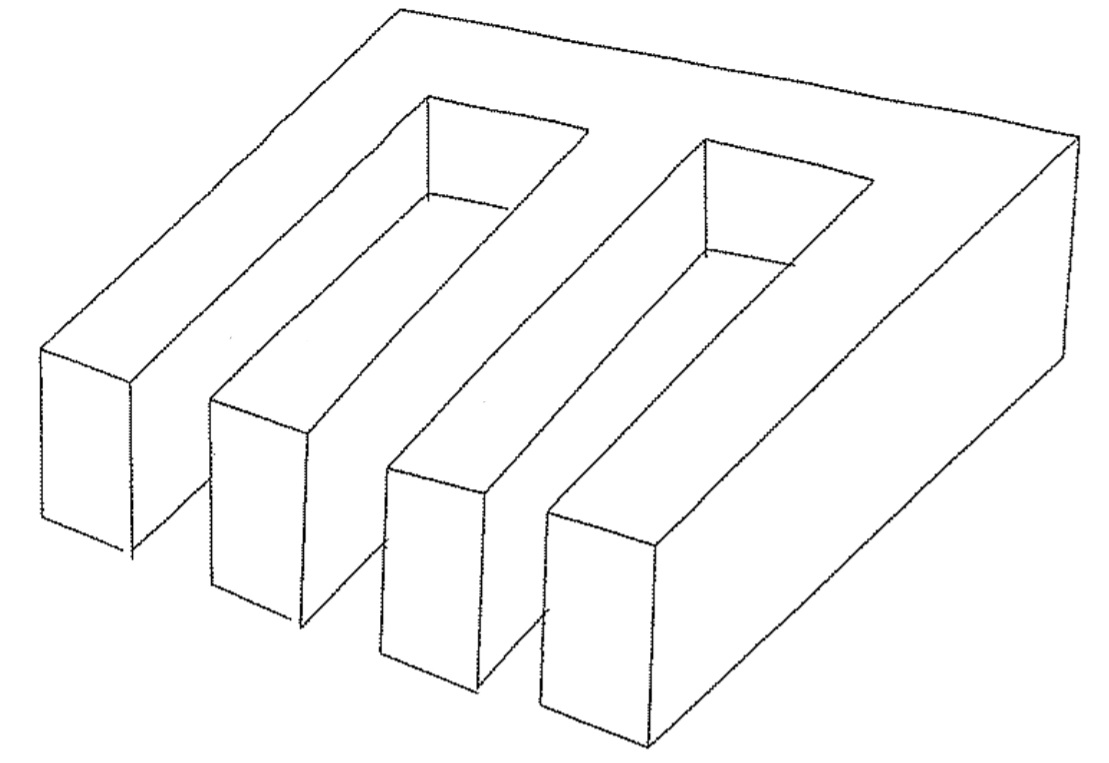
\includegraphics[scale=0.6]{m.jpg}
\end{center}

\clearpage
\tableofcontents

\clearpage
\section{Introducing the Course}
Introduction to two foundational concepts in cognitive science: representation of structures and its computation. Mechanistic explanation of structure.

\subsection{Description of the Course}
The course is an introduction to two foundational concepts in cognitive science: structural representations and computation. As empirical domain, we look at increasingly complex structural representations from morphology and syntax of natural languages. We couple this with an introduction to the theory of computation. We aim to establish that (i) human language capacity is (based on) a computationally describable unconscious system of rules and representations; (ii) that there are mathematically precise ways of talking about different types of structural relations; and (iii) that bringing these two together opens up new avenues in the cognitive scientific investigation of language. Natural language and linguistic knowledge. Language and grammar. Morphology. Syntax and grammatical structure. Semantics: Word meaning and grammatical meaning. Regular expressions and regular grammars. Push-down automata. An introduction to Parsing and derivation.
\subsection{Syllabus}
\begin{table}[H]
\renewcommand{\arraystretch}{1.5}
\begin{tabular}{|c l|}
\hline
Week & Topic                                   \\ \hline
1    & Introducing the Course                  \\ \hline
2    & Philosophical Premises and Fundamentals \\ \hline
3    & Formal Grammar                          \\ \hline
4    & Context-Free Grammar (CFG)              \\ \hline
5    & Regular Expressions                     \\ \hline
6    & Finite State Automata (FSA)             \\ \hline
7    & Removing Non-Determinism                \\ \hline
8    & Midterm Exam                            \\ \hline
9    & Lambda Calculus                         \\ \hline
10   & Lambda Calculus (Cont'd.)               \\ \hline
11   & Lambda Calculus (Still Cont'd.)         \\ \hline
12   & Push Down Automata (PDA)                \\ \hline
13   & Computational Uncertainty               \\ \hline
14   & Form, Meaning and Uncertainty in Computation               \\ \hline
15   & Final Exam                              \\ \hline
\end{tabular}
\end{table}
\clearpage

\section{Philosophical Premises and Fundamentals}
\subsection{Ambiguity}
Context is ambiguous but structure is not. However, there is structural ambiguity besides contextual ambiguity. The following sentence is ambiguous.
\begin{enumerate}
\item I saw the man with the telescope.\label{itm:tele}
\end{enumerate}
The sentence in (\ref{itm:tele}) has two interpretations as shown below.\\

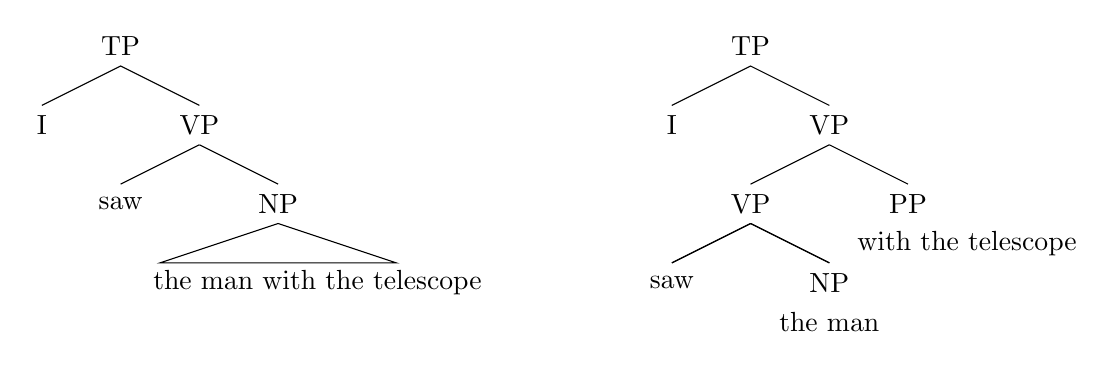
\begin{tikzpicture}
\draw (0,0) -- (1,0.5) -- (2,0);
\node at (1,0.75) {TP};
\draw (2,-0.5) -- (1,-1);
\node at (0,-0.25) {I};
\draw (2,-0.5) -- (3,-1);
\node at (2,-0.25) {VP};
\node at (1,-1.25) {saw};
\node at (3,-1.25) {NP};
\draw (3,-1.5) -- (1.5,-2) -- (4.5,-2) -- (3,-1.5);
\node at (3.5,-2.25) {the man with the telescope};

\draw (8,0) -- (9,0.5) -- (10,0);
\node at (9,0.75) {TP};
\draw (10,-0.5) -- (9,-1);
\node at (8,-0.25) {I};
\draw (10,-0.5) -- (11,-1);
\node at (10,-0.25) {VP};
\node at (9,-1.25) {VP};
\draw (9,-1.5) -- (8,-2);
\draw (9,-1.5) -- (10,-2);
\node at (11,-1.25) {PP};
\node at (11.75,-1.75) {with the telescope};
\draw (9,-1.5) -- (8,-2);
\draw (9,-1.5) -- (10,-2);
\node at (8,-2.25) {saw};
\node at (10,-2.75) {the man};
\node at (10,-2.25) {NP};

\end{tikzpicture}

The different interpretations derive from \emph{\textbf{locality}}; in other words, sisterhood relations of the phrases. However, it is worth noting that locality is not a physically local relation, yet it is a syntactic dependency relation. See the next sentence.
\begin{enumerate}
\setcounter{enumi}{1}
\item \textcolor{magenta}{Sen} \textcolor{blue}{benim} adamın kitabını okuduğu\textcolor{blue}{mu} sanıyor\textcolor{magenta}{sun}.\label{itm:sanı}
\end{enumerate}

The sentence in (\ref{itm:sanı}) shows that the structures with the same color are bound to each other although there is a physical distance between them.\\

\indent \textit{\textbf{Quick Note:} These explanations seem to be structural, but Structuralism in linguistics means the meticulous investigation of the structures in a language. In this regard, they are philological studies rather than linguistic studies as they don't bring an explanation specific to faculty of language. The process is to set rules and derive the language from these rules. However, in generative (Chomskian) linguistics, the rules (grammar) are directed by the language itself; i.e. language has rules that we cannot discover (we try at least), or can explain partially by revising throughout the time.}\\
\subsection{Formal Studies of Structures}
We are trying to come up with mechanisms for problems because rather than focusing on the input and output, we need to see the inside of the black box.\\
\begin{table}[H]
\centering
\begin{tabular}{c c}

\hline 
\underline{Mechanism} & \underline{Problem} \\ 
 
Simple & Simple \\ 

Complex & Complex \\ 
\hline
\end{tabular}
\caption{Marr's Type 1/2}
\label{tab:mech}
\end{table}

According to Table \ref{tab:mech}, the following statements are asserted. 
\begin{itemize}
\item If the problem and mechanism for that are simple, the job is easy.
\item If the problem is simple but mechanism is complex, this is not a proper way for science.
\item If the problem and mechanism are complex, this is \textbf{\emph{Type 2 theory}}.
\item If the problem is complex and the mechanism is simple, this is \emph{\textbf{Type 1 theory}}.
\end{itemize}

\indent \textit{\textbf{Quick Note:} There are two types of sorting: One is comparison sorting such as ordering the number from smaller to larger. The other is non-comparison sorting in which the elements are mapped onto a measure (I use the terms here fuzzily). For example, ordering people according to their height. In this case, height is mapped onto a computable value.}\\

\textbf{Marr's Levels\footnote{Marr, D. (1977). Artificial intelligence—a personal view. \textit{Artificial Intelligence, 9}(1), 37-48.}}
\begin{itemize}
\item Computational (goal, constraints, what and understanding the nature of the problem.)
\item Algorithmic (algorithms, data structures and representations.)
\item Implementation (how it is realized.)
\end{itemize}

\subsection{Formal Definitions}
\textit{\underline{Definition of Natural Numbers}}\\
$0 \in \mathbb{N}$\\
if $n \in \mathbb{N}$ then $_{s}(n) \in \mathbb{N}$\\
Nothing else is in $\mathbb{N}$\\

\noindent \textit{\underline{Definition of Even Natural Numbers}}\\
$f: 2n \rightarrow n$\\
f is 1-to-1,
f is onto,
f is total.\\

\textit{\textbf{Quick Note:} The set of $\mathbb{N}$ is an infinite set. Likewise, the set of even natural numbers is also infinite. However, when the sizes of these sets are asked to be compared, it can be intuitively said that one is half of the other, which is not the case, though. Instead, they are both of the same size (infinite).}\\
\begin{itemize}
\item A set is countable if it is equinumerous with some $n \in \mathbb{N}$. Any finite set is countable.
\item A set is countably infinite if it is equinumerous with $\mathbb{N}$.
\item A set $A$ is equinumerous with a set $B$ if there is a 1-to-1 correspondence from $A$ to $B$. $g: 2n+1 \rightarrow n$ if $n \in \mathbb{N}$
\end{itemize} 

\noindent \textbf{Complex problem:} Instances are too numerous to enumerate (but finite), search algorithm.
\subsection{Formal Language Theory}
Formal study of sets with properties is based on the idea that a well-formed (formal) coverage brings with the amount of computable resources needed.\\
\begin{figure}[H]
\centering
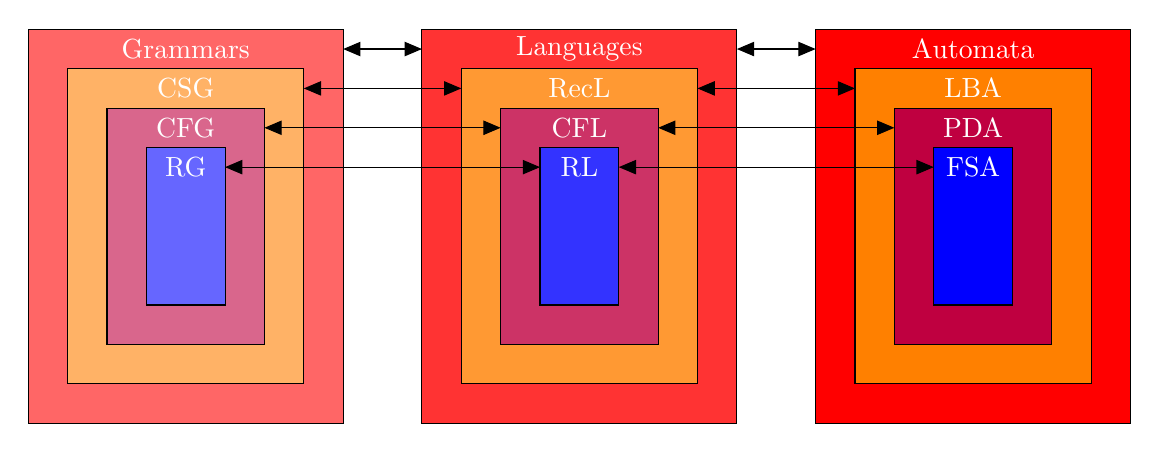
\begin{tikzpicture}
\draw[fill=red!60] (0,0) rectangle (4,5);
\draw[fill=orange!60] (0.5,0.5) rectangle (3.5,4.5);
\draw[fill=purple!60] (1,1) rectangle (3,4);
\draw[fill=blue!60] (1.5,1.5) rectangle (2.5,3.5);

\draw[fill=red!80] (5,0) rectangle (9,5);
\draw[fill=orange!80] (5.5,0.5) rectangle (8.5,4.5);
\draw[fill=purple!80] (6,1) rectangle (8,4);
\draw[fill=blue!80] (6.5,1.5) rectangle (7.5,3.5);

\draw[fill=red!100] (10,0) rectangle (14,5);
\draw[fill=orange!100] (10.5,0.5) rectangle (13.5,4.5);
\draw[fill=purple!100] (11,1) rectangle (13,4);
\draw[fill=blue!100] (11.5,1.5) rectangle (12.5,3.5);

\draw[>=triangle 45, <->] (4,4.75) -- (5,4.75);
\draw[>=triangle 45, <->] (3.5,4.25) -- (5.5,4.25);
\draw[>=triangle 45, <->] (3,3.75) -- (6,3.75);
\draw[>=triangle 45, <->] (2.5,3.25) -- (6.5,3.25);

\draw[>=triangle 45, <->] (9,4.75) -- (10,4.75);
\draw[>=triangle 45, <->] (8.5,4.25) -- (10.5,4.25);
\draw[>=triangle 45, <->] (8,3.75) -- (11,3.75);
\draw[>=triangle 45, <->](7.5,3.25) -- (11.5,3.25);

\node at (2,4.75) {\textcolor{white}{Grammars}};
\node at (7,4.75) {\textcolor{white}{Languages}};
\node at (12,4.75) {\textcolor{white}{Automata}};

\node at (2,4.25) {\textcolor{white}{CSG}};
\node at (7,4.25) {\textcolor{white}{RecL}};
\node at (12,4.25) {\textcolor{white}{LBA}};

\node at (2,3.75) {\textcolor{white}{CFG}};
\node at (7,3.75) {\textcolor{white}{CFL}};
\node at (12,3.75) {\textcolor{white}{PDA}};

\node at (2,3.25) {\textcolor{white}{RG}};
\node at (7,3.25) {\textcolor{white}{RL}};
\node at (12,3.25) {\textcolor{white}{FSA}};

\end{tikzpicture}
\caption{Schema of Grammars, Languages and Automata}
\end{figure}

\begin{table}[H]

\begin{tabular}{|c|c|c|c|}
\hline 
\textcolor{red}{Red} & Grammars & Languages & Automata \\ 

\textcolor{orange}{Orange} & Context-sensitive Grammar & Recursive Language & Linear-bound Automata \\ 

\textcolor{purple}{Purple} & Context-free Grammar & Context-free Language & Push-down Automata \\ 

\textcolor{blue}{Blue} & Regular Grammar & Regular Languages & Finite-state Automata \\ 
\hline 
\end{tabular}
\caption{Languages, Grammars and Automata and their counterparts }
\end{table}

\indent \textit{\textbf{Quick Note:} Recursible enumerable languages can be completed by Turing machine. Anything finite is regular. Halting problem (loop) is an unrestricted problem.}\\\\

\noindent \textbf{\Large{QUIZ 1:}}\\
$L = \lbrace I, think, you, like \rbrace $\\
mini English = Every grammatical sentence in English.\\
Show that mini English is a countably infinite set.\\

\noindent \textbf{\Large{Answer:}}\\
Let $l(n) = $ length of sentence $S$\\
$f(2n+3) = n$ where 0 maps onto 3, 1 maps onto 5, 2 maps onto 7 and so on.\\
This proves that $f$ is 1-1. However, the problem is the sentences which are of the same length such as \textit{``You think I like you"} and \textit{``I think I like you"} whose lengths are 5. The solution is:\\
Let $g(n)=$ set of all sentences in mini English that are of the length $n$.\\
$A = \lbrace$\textit{I think I like you, You think I like you} $\rbrace$\\
$g(5)$ maps onto 0, $g(7)$ maps onto 1, $g(9)$ maps onto 2, $g(11)$ maps onto 3 and so on. All those $g$ functions in total constitute mini English.\\
Let $h(g(2n+3)) = n$, $h$ is 1-1 correspondence. $B = \lbrace$ \textit{``I like you"}, \textit{``You like you"} $\rbrace$\\

\indent \textit{\textbf{Quick Note:} We need to make a formal definition first, then make the empirical justification.}

\clearpage

\section{Formal Grammar}
\subsection{Formalism and Relation}
\textbf{\emph{Formal grammar}} means two things: Study of formal forms in grammar and the rigorous study of grammar (empirical).\\
Relation is, different from a function, one to many.\\

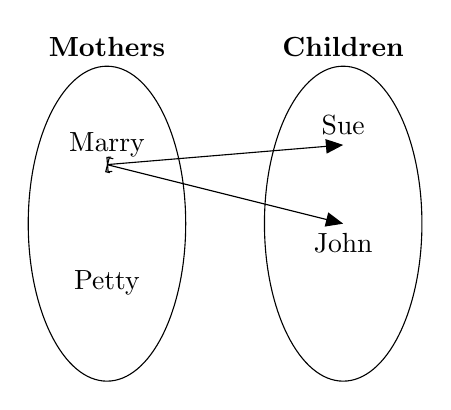
\begin{tikzpicture}
\draw (0,0) ellipse (1cm and 2cm);
\draw (3,0) ellipse (1cm and 2cm);
\draw[>=triangle 45, [->] (0,0.75) -- (3,1);
\draw[>=triangle 45, [->] (0,0.75) -- (3,0);
\node at (0,1) {Marry};
\node at (0,-0.75) {Petty};
\node at (3,-0.25) {John};
\node at (3,1.25) {Sue};
\node at (0,2.25) {\textbf{Mothers}};
\node at (3,2.25) {\textbf{Children}};
\end{tikzpicture}\\

\textit{\textbf{Quick Note:} Not every element in the domain set has to have a correspondence in the range. The mathematical notation of the relation given is: $\langle$ \emph{Mary, Sue} $\rangle$ $\in$ \emph{mother of} or \emph{Mary mother of John}.}\\

\noindent $l(n)$ is an equivalent relation on the length of sentences. An equivalent relation is reflexive, symmetric and transitive.\\

\noindent \textbf{\underline{Reflextive :}} If $x$ $\in$ $domain(R)$ and $y$ $\in$ $range(R)$, then $x$ $R$ $y$ and $y$ $R$ $x$ hold. \\
\textbf{\underline{Symmetric:}} If $x$ $\in$ $domain(R)$ then $x$ $R$ $x$ holds.\\
\textbf{\underline{Transitive :}} If $x$ $R$ $y$ and $y$ $R$ $z$ then $x$ $R$ $z$ holds.

\subsection{Formal Study of Structure in mini English}
$\Big[$ I think $\big[$ I like you $\big]$ $_{Clause}$ $\Big]$ $_{Clause}$\\

\textbf{First Try:} All predicates take a subject, but not all predicates take an object.\\
I think I like you.\\
$^{\ast}$I like I like you.\\
$^{\ast}$I like I think you.\\

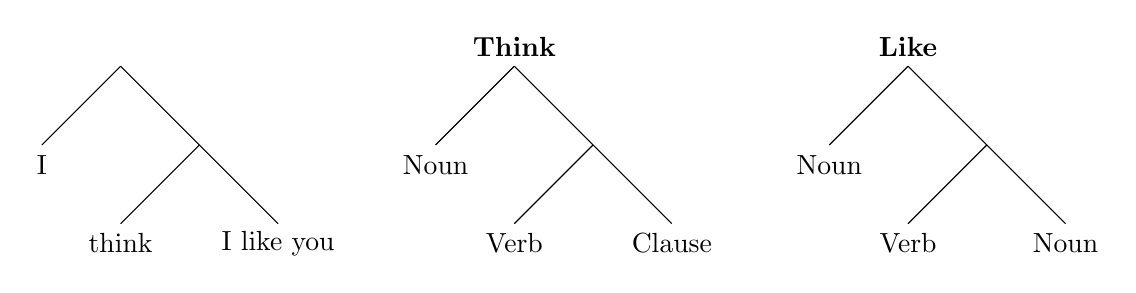
\begin{tikzpicture}
\draw (0,0) -- (1,1);
\draw (1,1) -- (2,0);
\draw (2,0) -- (1,-1);
\draw (2,0) -- (3,-1);
\node at (0,-0.25) {I};
\node at (1,-1.25) {think};
\node at (3,-1.25) {I like you};

\draw (5,0) -- (6,1);
\draw (6,1) -- (7,0);
\draw (7,0) -- (6,-1);
\draw (7,0) -- (8,-1);
\node at (5,-0.25) {Noun};
\node at (6,-1.25) {Verb};
\node at (8,-1.25) {Clause};
\node at (6,1.25) {\textbf{Think}};

\draw (10,0) -- (11,1);
\draw (11,1) -- (12,0);
\draw (12,0) -- (11,-1);
\draw (12,0) -- (13,-1);
\node at (10,-0.25) {Noun};
\node at (11,-1.25) {Verb};
\node at (13,-1.25) {Noun};
\node at (11,1.25) {\textbf{Like}};
\end{tikzpicture}\\
\clearpage
\textbf{Second Try:} I think you think I think I like you.\\

\begin{tikzpicture}
\draw (0,0) -- (1.5,0.50) -- (3,0);
\node at (1.5,0.75) {S};
\node at (0,-0.25) {I};
\draw (1.5,-1) -- (3,-0.5) -- (4.5,-1);
\node at (3,-0.25) {VP};
\node at (1.5,-1.25) {think};
\draw (3,-2) -- (4.5,-1.5) -- (6,-2);
\node at (4.5,-1.25) {S};
\node at (3,-2.25) {you};
\draw (4.5,-3) -- (6,-2.5) -- (7.5,-3);
\node at (6,-2.25) {VP};
\node at (4.5,-3.25) {think};
\draw (6,-4) -- (7.5,-3.5) -- (9,-4);
\node at (7.5,-3.25) {S};
\node at (6,-4.25) {I};
\draw (7.5,-5) -- (9,-4.5) -- (10.5,-5);
\node at (9,-4.25) {VP};
\node at (7.5,-5.25) {think};
\draw (9,-6) -- (10.5,-5.5) -- (12,-6);
\node at (10.5,-5.25) {S};
\node at (9,-6.25) {I};
\draw (10.5,-7) -- (12,-6.5) -- (13.5,-7);
\node at (12,-6.25) {VP};
\node at (10.5,-7.25) {like};
\node at (13.5,-7.25) {you};
\end{tikzpicture}\\


\textbf{Third Try:} A phrase Structure Grammar of mini English\\
S $\rightarrow$ NP VP\\
NP $\rightarrow$ I\\
NP $\rightarrow$ you\\
VP $\rightarrow$ V NP\\
VP $\rightarrow$ V S\\
V $\rightarrow$ like\\
V $\rightarrow$ think

\begin{table}[H]
\begin{tabular}{c}
\hline 
\emph{\textbf{Grammar}} is a set of rules. \\ 
\hline 
\end{tabular} 
\end{table}

\textbf{Empirical Problems:}
\begin{itemize}
\item \textit{``I like I think you"} is bad but grammar says it is OK.
\item \textit{``You like I"} is also OK for grammar.
\end{itemize}

\textbf{Fourth Try:}\\
V$_{tv}$ $\rightarrow$ like\\
V$_{psych}$ $\rightarrow$ think\\
VP $\rightarrow$ V$_{tv}$ NP$_{acc}$ \\
VP $\rightarrow$ V$_{psych}$ S\\
NP$_{nom}$ $\rightarrow$ You (nominative)\\
NP$_{acc}$ $\rightarrow$ You (accusative)\\
S $\rightarrow$ NP$_{nom}$ VP\\
NP$_{nom}$ $\rightarrow$ I

\subsection{Grammars}
A \emph{\textbf{phrase structure grammar (PSG)}} is the one which all rules can be drawn as trees (phrase markers). Phrase markers are empirical generalizations.\\
\noindent A \emph{\textbf{context-free grammar (CFG)}} is a PSG in which we have formal symbols, and siblings are ordered.\\

\emph{\underline{\textbf{Definitions:}}}\\

Let $G=(V, \Sigma, R, S)$\\
$V$: Set of variables (unknowns)\\
$\Sigma$: Set of invariables \\
$R$: Set of rules\\
$S$: Start symbol ($s \in V$)\\

\noindent a \textbf{\emph{CFG}} is where all rules in $R$ are $\alpha \rightarrow \beta$;\\
if $\alpha \in V$ and $\beta \in (V \cup \Sigma)^{\ast}$\\
then $\alpha$\\
\begin{tikzpicture}
\draw [color=white](1,0) -- (3.75,-0.7);
\draw (2,-0.05) -- (1.8,-0.75);
\end{tikzpicture}\\
\indent $\beta$ is a tree.

\subsection{Sets and Concatenations}
Let $A$ and $B$ sets, $A \cup B$, $A \cap B$, $A-B$, $AB \rightarrow$ set concatenation.\\
For example, $A = \lbrace 0,1,2 \rbrace$ and $B= \lbrace a,b,c \rbrace$; $AB= \lbrace 0a,0b,0c,1a,1b,1c,2a,2b,2c \rbrace$\\

\noindent \emph{\underline{\textbf{Definition:}}}\\
$AB = \lbrace x_{1}, x_{2} | x_{1} \in A, x_{2} \in B \rbrace$\\
Concatenation of $A$, $A^{\ast} = A^{0} \cup A^{1} \cup A^{2} \cdots \cup A^{i}$ \\

\begin{table}[H]
\centering
\begin{tabular}{cc}
\hline 
\emph{``What is math? Algebra, Calculus. That's it!"} & \\

 & (Bozşahin)\\
\hline 
\end{tabular} 
\end{table}

$A^{0}=\lbrace e \rbrace$ and $\forall A$, $A^{0} \neq \emptyset$\\

\noindent \underline{\textbf{Example:}}\\
S $\rightarrow$ NP VP\\
VP $\rightarrow$ V NP\\
VP $\rightarrow$ V S\\
NP $\rightarrow$ I $\mid$ You\\

\noindent Variables= $\lbrace S,VP,ZP,V \rbrace$\\
$\Sigma= \lbrace I,like,you,think \rbrace$\\
$R= \lbrace S \rightarrow$ $NP$ $VP$, $VP \rightarrow$ $V$ $NP$ $\rbrace$\\

\textit{\textbf{Quick Note:} $V \rightarrow non-terminals$, $\Sigma \rightarrow$ $alphabet$ $terminals$}\\
\clearpage
\noindent \textbf{\Large{QUIZ 2:}}\\
Write a context-free grammar defined over the alphabet $\Sigma = \lbrace 0,1 \rbrace$ such that all the strings start with 0 and end with 0. For instance, $``010110"$ $\in L_{1}$ but $``100010"$ $\notin L_{1}$.\\

\noindent \textbf{\Large{Answer:}}\\
$L=$ set of strings in $\Sigma^{*}$ that start and end with $0$.\\
$L_{1}$ start and end with with different $0$s.\\
$L_{1}$ start and end with with the same $0$, which includes the string $``0"$\\

Grammar for $L_{1}$: All and only the strings in $L_{1}$ (completeness and soundness).\\
$G_{1}$: $S \rightarrow 0A0$, $A \rightarrow 0A | 1A | \varepsilon$\\
$G_{2}$: $S \rightarrow 0B$, $B \rightarrow C0 | \varepsilon$, $C\rightarrow C | 0C | \varepsilon$\\

\begin{tikzpicture}
\draw (0,0) -- (1.5,0.50) -- (3,0);
\node at (1.5,0.75) {S};
\node at (0,-0.25) {$0$};
\node at (3,-0.25) {$0$};
\draw (1.5,0.5) -- (1.5,0);
\node at (1.5,-0.25) {$A$};
\draw (1.5, -0.5) -- (1.5,-1);
\node at (1.5,-1.25) {$\varepsilon$};

\draw (5,0) -- (6.5,0.50) -- (8,0);
\node at (6.5,0.75) {S};
\node at (8,-0.25) {$B$};
\node at (5,-0.25) {$0$};
\draw (8,-0.5) -- (8,-1);
\node at (8,-1.25) {$\varepsilon$};
\end{tikzpicture}\\

\noindent The first tree generated with $G_{1}$ does not accept the string which starts and ends with the same $0$. However, the second tree generated with $G_{2}$ solves the problem.

\clearpage

\section{Context-Free Grammars}
\subsection{Problem of Computation}
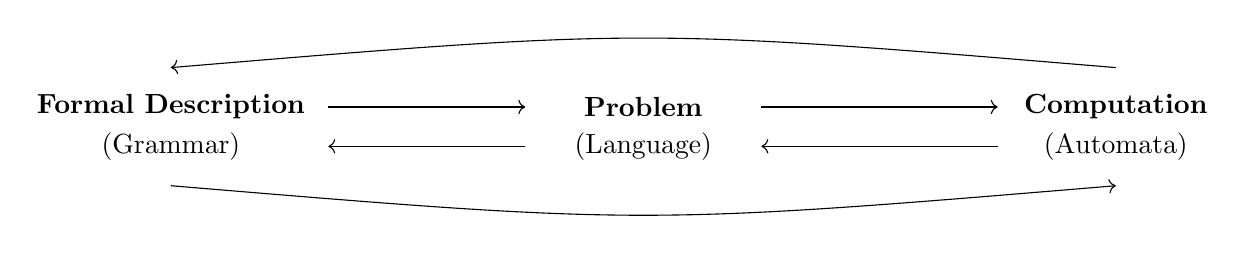
\begin{tikzpicture}
\node at (0,0){\textbf{Formal Description}};
\node at (0,-0.5){(Grammar)};
\node at (6,0){\textbf{Problem}};
\node at (6,-0.5){(Language)};
\node at (12,0){\textbf{Computation}};
\node at (12,-0.5){(Automata)};
\draw[->] (2,0) -- (4.5,0);
\draw[->] (4.5,-0.5) -- (2,-0.5);
\draw[->] (7.5,0) -- (10.5,0);
\draw[->] (10.5,-0.5) -- (7.5,-0.5);
\draw[->] (0,-1) .. controls (6,-1.5) .. (12,-1);
\draw[<-] (0,0.5) .. controls (6,1) .. (12,0.5);
\end{tikzpicture}\\

Grammar rules $\alpha\rightarrow\beta$ ($\alpha$ is $\beta$, $\alpha$ rewrites $\beta$). If $|\alpha|=1$ then we have a CFG (gives us a tree).\\

\textbf{$G=\lbrace V,\Sigma,R,S\rbrace$}

\subsection{Languages and Grammars}
Let $L_{2}$ has the grammar $G_{2}$ which has the phrase markers $S\rightarrow0A$, $A\rightarrow0A|1B|\varepsilon$, $B\rightarrow0A|1B$, show that the string \emph{``011"} is not a string that can be generated with $G_{2}$ in parse tree.\\

\begin{tikzpicture}
\draw (0,0) -- (1.5,0.50) -- (3,0);
\node at (1.5,0.75) {S};
\node at (0,-0.25) {$0$};
\node at (3,-0.25) {$A$};
\draw (1.5,-1) -- (3,-0.5) --(4.5,-1);
\node at (1.5,-1.25){$1$};
\node at (4.5,-1.25){$B$};
\draw (4.5,-1.5) -- (2.5,-2) -- (6.5,-2)-- (4.5,-1.5);
\end{tikzpicture}\\

\noindent This tree will never generate the above-mentioned string. Similarly, the grammar of the language in \textbf{Quiz 2} behaves the same. Therefore, although the string is the same, structure is different, which indicates that \emph{if $L_{1}$ and $L_{2}$ are not the same, then they cannot have equivalent grammars. For a given language, there can be many equivalent grammars.}\\

\underline{\textbf{Definition:}}\\
$G_{1}$ and $G_{2}$ are weakly equivalent: $f:$ $L(G_{1})=L(G_{2})$\\

\noindent \underline{\textbf{Example:}}\\
Let the language $L_{3}$ have the alphabet $\Sigma= \lbrace a,b \rbrace$. That language includes all strings where $a$s do not follow $b$s.\\

$\varepsilon,a,b,ab$ $\in$ $L_{3}$ and $ba,aabba$ $\notin$ $L_{3}$\\

\textbf{$S \rightarrow A$ $B$, $A \rightarrow aA|\varepsilon$, $B\rightarrow bB|\varepsilon$} \textbf{(Divide and Conquer!)}\\

\textit{\textbf{Quick Note: }Only regular languages have unique description.}\\

\clearpage

\noindent \underline{\textbf{Example:}}\\
Let the language $L_{4}$ have the alphabet $\Sigma= \lbrace a,b \rbrace$. That language includes all strings where the number of $a'$s is equal to that of $b'$s.

\begin{enumerate}
\item $G_{4}^{'}:$ $S \rightarrow aSb|\varepsilon$
\item $G_{4}^{''}:$ $S \rightarrow A$, $A \rightarrow aB|\varepsilon$, $B\rightarrow Ab|b$
\end{enumerate}

\noindent \textbf{\Large{QUIZ 3:}}\\
Let the language $L_{5}$ have the alphabet $\Sigma= \lbrace a,b,c \rbrace$. That language includes all strings where there are twice as many $b'$s as $a'$s ($L_{5}=\lbrace a^{n}cb^{2n}\rbrace$). Write the grammar of $L_{5}$.\\


\noindent \textbf{\Large{Answer:}}\\
$S\rightarrow$ $aSbb$ $|$ $c$\\

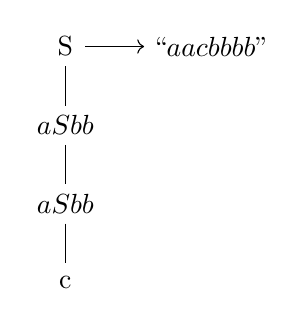
\begin{tikzpicture}
\draw (0,0) -- (0,0.5);
\node at (0,0.75) {S};
\node at (0,-0.25) {$aSbb$};
\draw (0,-0.50) -- (0,-1);
\node at (0,-1.25) {$aSbb$};
\draw (0,-1.50) -- (0,-2);
\node at (0,-2.25) {c};
\draw[->] (0.25,0.75) -- (1,0.75);
\node at (1.85,0.75) {$``aacbbbb"$};
\end{tikzpicture}\\

\clearpage

\section{Regular Expressions}
\subsection{Language of a Grammar}
Language of a grammar is $L(G)=\lbrace x$ $|$ $x$ $\in$ $\Sigma^{*}$, $S\overset{*}{\Rightarrow}x\rbrace$\\

\textit{\textbf{Quick Note:} Double arrow indicates \textbf{use of a rule}.}\\

\noindent \underline{\textbf{Example:}}\\
$acbb$ $\in$ $L$\\

\begin{tikzpicture}
\draw (0,0) -- (1.5,0.50) -- (3,0);
\node at (1.5,0.75) {S};
\node at (0,-0.25) {$a$};
\node at (3,-0.25) {$A$};
\draw (1.5,-1) -- (3,-0.5) --(4.5,-1);
\node at (1.5,-1.25){$S$};
\draw (3,-0.5) -- (3,-1);
\node at (4.5,-1.25){$b$};
\node at (3,-1.25){$b$};
\draw (1.5,-1.5) -- (1.5,-2);
\node at (1.5,-2.25){$c$};
\end{tikzpicture}\\

\textbf{$S\overset{1}{\Rightarrow}aA\overset{2}{\Rightarrow}aSbb\overset{3}{\Rightarrow}acbb$}\\

\noindent $abb$ $\notin$ $L$\\
{$S\overset{1}{\Rightarrow}aA\overset{2}{\Rightarrow}aSbb$, this is not going to lead you to the desired string.

\subsection{Different Languages and Grammars}
1 counter\textcolor{white}{s} $L_{1}=$ $\lbrace a^{n},$ $b^{n}\rbrace$\\
2 counters $L_{2}=$ $\lbrace a^{n},$ $b^{m},$ $c^{m},$ $b^{n}\rbrace$\\
3 counters $L_{2}=$ $\lbrace a^{n},$ $b^{m},$ $c^{a},$ $r^{a},$ $c^{m},$ $b^{n}\rbrace$\\

\textbf{No matter how many counters there are, the problem is the same.}\\

\noindent $S_{1}\rightarrow aS_{1}b|\epsilon$\\
$S_{2}\rightarrow aS_{2}b|A$, $A\rightarrow bAc | \epsilon$\\
$S_{3}\rightarrow aS_{3}b |A$, $A\rightarrow bAc| B$, $B\rightarrow cBr | \epsilon$\\

\textbf{BUT the real problem is something different.}\\

\begin{enumerate}
\item $\lbrace a^{n}b^{m}|n,m\geq0\rbrace$
\item $\lbrace a^{n}b^{n}|n\geq0\rbrace$
\item $\lbrace a^{n}b^{n}c^{n}|n\geq0\rbrace$
\end{enumerate}

\begin{enumerate}
\item $G_{1}$: $S\rightarrow aS|A,$ $A\rightarrow bA|\epsilon$
\item $G_{2}$: $S\rightarrow aSb|c$
\item \emph{No context-free grammar for this!}
\end{enumerate}

Some problems \emph{($\equiv$ languages $\equiv$ sets with structure)} are easy enough so that multiple descriptions can be captured by a unique automaton \emph{(Regular expressions)}. Some problems are more resource demanding, so there is no guarantee for unique computation.\\

$L=\lbrace a^{i}|$ $i$ \emph{is a prime number.}$\rbrace$ $\longrightarrow$ \textbf{impossible to write a CFG for this problem.}\\

\emph{\textbf{Regular languages}} are \underline{a proper subset} of context-free languages. There is a regular grammar for every language. A grammar is regular if all rules are of tree forms $A\rightarrow aB$ (right regular) or $A\rightarrow Ba$ (left regular).

\subsection{Regular Expressions (Regexp)}
Let $\Sigma=\lbrace a,b\rbrace$
\begin{enumerate}
\item For $\forall a$ $\in$ $\Sigma \cup\lbrace\epsilon\rbrace$, $\alpha$ is a regular expression.
\item If $\alpha$, $\beta$ are regular expressions, then $\alpha\beta$ (concatenation of two expressions), $\alpha\cup\beta$ (union of two expressions), $\alpha^{*}$ (k-star) are regular expressions as well.
\item Nothing else generated without \emph{(1)} and \emph{(2)} are regular expression. 
\end{enumerate}

\noindent \underline{\textbf{Example 1:}}\\
$\lbrace a^{n}b^{m}|n,m\geq 0\rbrace$\\
\textbf{Regexp:} $a^{*}b^{*}$\\

\noindent \underline{\textbf{Example 2:}}\\
A language where no $a$ follows $b$.\\
\textbf{Regexp:} $a^{*}b^{*}$\\

\noindent \underline{\textbf{Example 3:}}\\
$\Sigma=\lbrace a,b,c\rbrace$, All and only strings without the substring $bb$.\\
\textbf{Regexp:} $(a|c|b(a|c))^{*}(b|\epsilon)$

\begin{table}[H]
\centering
\begin{tabular}{cc}
\hline 
\emph{Math is as useful as art. Math is black art.} &\\ 
& (Bozşahin) \\ 
\hline 
\end{tabular} 
\end{table}

\textit{\textbf{Quick Note:} $\alpha^{+}=\alpha\alpha^{*}\longrightarrow$ \textbf{at least one} $alpha$.}\\

\noindent \underline{\textbf{Example 4:}}\\
$\Sigma=\lbrace 0,1\rbrace$, $L=$ All and only strings in $\Sigma^{*}$ where every third symbol is $1$.\\
\textbf{Regexp:} $((0|1)(0|1)1)^{*}(0|1|\epsilon)^{2}$\\

\noindent \underline{\textbf{Example 5:}}\\
$\Sigma=\lbrace a,b,c\rbrace$, $L=$ All and only strings that do not contain the substring $ac$.\\
\textbf{Regexp:} $(b|c|a^{*}b)^{*}(a|b)^{*}$\\

\textit{\textbf{Quick Note:} If $X\subseteq Y$ and $Y\subseteq X$, then $X=Y$. \emph{$X$ and $Y$ are countably infinite.}}

\begin{table}[H]
\centering
\begin{tabular}{cc}
\hline 
\emph{Grammars give you ``what", Automata give you ``how".} &\\ 
& (Bozşahin) \\ 
\hline 
\end{tabular} 
\end{table}

\noindent \underline{\textbf{Example 5:}}\\
$\Sigma = \lbrace \llcorner , \urcorner , c \rbrace$, All and only squares out of $\Sigma$.\\
\textbf{Regexp:} $(\llcorner \urcorner c)^{*}$\\

\noindent \textbf{\Large{QUIZ 4:}}\\
Let $\Sigma=\lbrace a,b,c\rbrace$, given $L=$ All and only strings with even number of $a$'s.\\

\noindent \textbf{\Large{Answer:}}\\
$((b|c)^{*}(a(b|c)^{*}a)^{*}(b|c)^{*})^{*}$
\clearpage

\section{Finite State Automata}
\subsection{From Description to Computation}
\underline{Theorem}\\
For every language, there is a finite state automaton that computes its strings.\\
For every regular language, there is a regular expression.\\
For every regular language, there is a regular grammar.\\

\noindent A \textbf{\emph{finite state automaton (FSA)}} is a mathematical model of computation. It is an abstract machine that can be in exactly one of a finite number of states at any given time.\footnote{\url{https://en.wikipedia.org/wiki/Finite-state_machine}}\\

$M=\langle Q,\Sigma , \Delta ,q_{0}(s) ,F \rangle$\\

\noindent $Q$: Finite set of states\\
$\Sigma$: Alphabet\\
$\Delta$: Finite set of transitions\\
$q_{0}$: Start state $q_{0} \in Q$\\
$F$: Set of final (accepting) states $F \subseteq Q$\\

\underline{\textbf{Example}}\\
$M_{1}$: All and only strings with even number of \emph{a}'s.\\

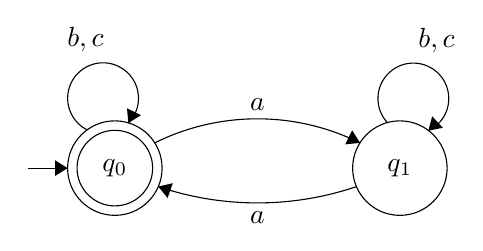
\begin{tikzpicture}[scale=0.2]
\tikzstyle{every node}+=[inner sep=0pt]
\draw [black] (20.9,-21.3) circle (3);
\draw (20.9,-21.3) node {$q_{0}$};
\draw [black] (20.9,-21.3) circle (2.4);
\draw [black] (39,-21.3) circle (3);
\draw (39,-21.3) node {$q_{1}$};
\draw [black] (23.431,-19.7) arc (116.42945:63.57055:14.645);
\fill [black] (36.47,-19.7) -- (35.97,-18.9) -- (35.53,-19.79);
\draw (29.95,-17.67) node [above] {$a$};
\draw [black] (36.243,-22.475) arc (-71.3017:-108.6983:19.629);
\fill [black] (23.66,-22.47) -- (24.25,-23.2) -- (24.58,-22.26);
\draw (29.95,-24.01) node [below] {$a$};
\draw [black] (15.4,-21.3) -- (17.9,-21.3);
\fill [black] (17.9,-21.3) -- (17.1,-20.8) -- (17.1,-21.8);
\draw [black] (19.151,-18.877) arc (243.55053:-44.44947:2.25);
\draw (19.03,-13.98) node [above] {$b,c$};
\fill [black] (21.76,-18.44) -- (22.56,-17.94) -- (21.67,-17.5);
\draw [black] (38.212,-18.417) arc (223.02275:-64.97725:2.25);
\draw (41.33,-14) node [above] {$b,c$};
\fill [black] (40.81,-18.92) -- (41.73,-18.74) -- (41.05,-18.01);
\end{tikzpicture}\\

$M_{1}=( \lbrace q_{0},q_{1} \rbrace, \lbrace a,b,c \rbrace , \lbrace \lbrace q_{0},a,q_{0}\rbrace\lbrace q_{0},b,q_{1}\rbrace\lbrace q_{0},c,q_{1}\rbrace\lbrace q_{1},a,q_{0}\rbrace\lbrace q_{1},b,q_{0}\rbrace\lbrace q_{1},c,q_{0}\rbrace \rbrace ,q_{0} ,  \lbrace q_{0}\rbrace)$\\

\noindent \textbf{One-step computation} ($\vdash$): how we advance the configuration \emph{(all pieces of information needed)} of computation.\\
Call \emph{(q,w)} a \textbf{configuration} of an fa \emph{M}, where \emph{q} is the current state and \emph{w} is the string on the tape including the current symbol and what lies to the right of it.\footnote{Umut Özge, COGS501 Lecture Notes}\\

A configuration \emph{(q,w)} is such that $p \in Q$ and $w \in (\Sigma \cup (\lbrace \epsilon \rbrace)^{*}$\\

\noindent \textbf{Initial Configuration:} \emph{(s, input)}\\
\textbf{Accepting Configuration:} \emph{(p, $\epsilon$)} if $p \in F$\\

\emph{L(M)}, language of a machine, $M$=$\lbrace x|x \in \Sigma^{*}$ and $(s,x)\overset{*}{\vdash}(p,\epsilon)$ $p \in F$\\

\underline{\textbf{Use of ``$\vdash$"}}\\
$a \in \Sigma$, $w\in \Sigma^{*}$ $(r, a, w)\vdash (q,w)$ if $(r,a,q)\in \Delta $\\

\underline{\textbf{Example}}\\
$L_{1}=$ All and only strings where every third symbol is \emph{a}.\\

$(a|b)(a|b)a)^{*}(a|b|\epsilon)^{2}$
\begin{center}
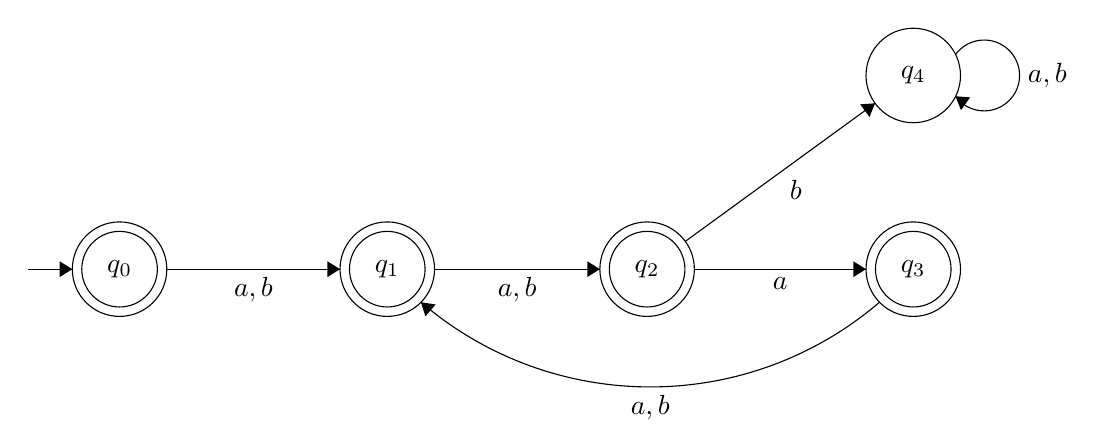
\begin{tikzpicture}[scale=0.2]
\tikzstyle{every node}+=[inner sep=0pt]
\draw [black] (14.6,-21.6) circle (3);
\draw (14.6,-21.6) node {$q_{0}$};
\draw [black] (14.6,-21.6) circle (2.4);
\draw [black] (31.6,-21.6) circle (3);
\draw (31.6,-21.6) node {$q_{1}$};
\draw [black] (31.6,-21.6) circle (2.4);
\draw [black] (48.1,-21.6) circle (3);
\draw (48.1,-21.6) node {$q_{2}$};
\draw [black] (48.1,-21.6) circle (2.4);
\draw [black] (65,-21.6) circle (3);
\draw (65,-21.6) node {$q_{3}$};
\draw [black] (65,-21.6) circle (2.4);
\draw [black] (65,-9.3) circle (3);
\draw (65,-9.3) node {$q_{4}$};
\draw [black] (17.6,-21.6) -- (28.6,-21.6);
\fill [black] (28.6,-21.6) -- (27.8,-21.1) -- (27.8,-22.1);
\draw (23.1,-22.1) node [below] {$a,b$};
\draw [black] (34.6,-21.6) -- (45.1,-21.6);
\fill [black] (45.1,-21.6) -- (44.3,-21.1) -- (44.3,-22.1);
\draw (39.85,-22.1) node [below] {$a,b$};
\draw [black] (51.1,-21.6) -- (62,-21.6);
\fill [black] (62,-21.6) -- (61.2,-21.1) -- (61.2,-22.1);
\draw (56.55,-22.1) node [below] {$a$};
\draw [black] (50.53,-19.83) -- (62.57,-11.07);
\fill [black] (62.57,-11.07) -- (61.63,-11.13) -- (62.22,-11.94);
\draw (57.55,-15.95) node [below] {$b$};
\draw [black] (67.68,-7.977) arc (144:-144:2.25);
\draw (72.25,-9.3) node [right] {$a,b$};
\fill [black] (67.68,-10.62) -- (68.03,-11.5) -- (68.62,-10.69);
\draw [black] (62.859,-23.698) arc (-49.43062:-130.56938:22.385);
\fill [black] (33.74,-23.7) -- (34.02,-24.6) -- (34.67,-23.84);
\draw (48.3,-29.58) node [below] {$a,b$};
\draw [black] (8.8,-21.6) -- (11.6,-21.6);
\fill [black] (11.6,-21.6) -- (10.8,-21.1) -- (10.8,-22.1);
\end{tikzpicture}
\end{center}

\underline{\textbf{Example}}\\
$L_{1}=$ All and only strings with even number of \emph{0}'s and odd number of \emph{1}'s.\\
$\Sigma=\lbrace 0,1 \rbrace$\\

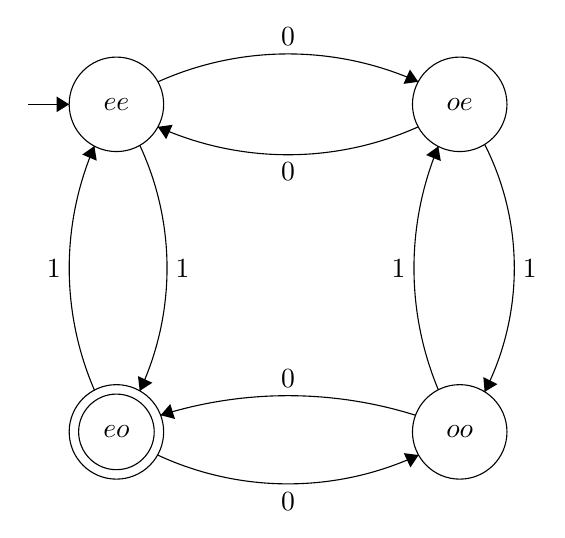
\begin{tikzpicture}[scale=0.2]
\tikzstyle{every node}+=[inner sep=0pt]
\draw [black] (16,-19.4) circle (3);
\draw (16,-19.4) node {$ee$};
\draw [black] (16,-40.2) circle (3);
\draw (16,-40.2) node {$eo$};
\draw [black] (16,-40.2) circle (2.4);
\draw [black] (37.8,-19.4) circle (3);
\draw (37.8,-19.4) node {$oe$};
\draw [black] (37.8,-40.2) circle (3);
\draw (37.8,-40.2) node {$oo$};
\draw [black] (10.4,-19.4) -- (13,-19.4);
\fill [black] (13,-19.4) -- (12.2,-18.9) -- (12.2,-19.9);
\draw [black] (17.484,-22.003) arc (25.02984:-25.02984:18.428);
\fill [black] (17.48,-37.6) -- (18.28,-37.08) -- (17.37,-36.66);
\draw (19.72,-29.8) node [right] {$1$};
\draw [black] (14.604,-37.548) arc (-156.63549:-203.36451:19.537);
\fill [black] (14.6,-22.05) -- (13.83,-22.59) -- (14.75,-22.98);
\draw (12.5,-29.8) node [left] {$1$};
\draw [black] (18.635,-17.971) arc (114.20509:65.79491:20.159);
\fill [black] (35.17,-17.97) -- (34.64,-17.19) -- (34.23,-18.1);
\draw (26.9,-15.7) node [above] {$0$};
\draw [black] (35.165,-20.829) arc (-65.79491:-114.20509:20.159);
\fill [black] (18.63,-20.83) -- (19.16,-21.61) -- (19.57,-20.7);
\draw (26.9,-23.1) node [below] {$0$};
\draw [black] (39.384,-21.943) arc (26.95437:-26.95437:17.333);
\fill [black] (39.38,-37.66) -- (40.19,-37.17) -- (39.3,-36.72);
\draw (41.77,-29.8) node [right] {$1$};
\draw [black] (36.442,-37.528) arc (-157.34631:-202.65369:20.064);
\fill [black] (36.44,-22.07) -- (35.67,-22.62) -- (36.6,-23);
\draw (34.39,-29.8) node [left] {$1$};
\draw [black] (18.806,-39.143) arc (107.46027:72.53973:26.976);
\fill [black] (18.81,-39.14) -- (19.72,-39.38) -- (19.42,-38.43);
\draw (26.9,-37.4) node [above] {$0$};
\draw [black] (35.187,-41.668) arc (-65.05212:-114.94788:19.647);
\fill [black] (35.19,-41.67) -- (34.25,-41.55) -- (34.67,-42.46);
\draw (26.9,-44) node [below] {$0$};
\end{tikzpicture}

\indent \textit{\textbf{Quick Note:} In deterministic finite automata, the next configuration is just one, in non-deterministic automata (NFA); on the other hand, there are more than one configuration. NFA give you expressivity but no extra power.}\\

\underline{\textbf{Example}}\\
\begin{enumerate}
\item $\overset{\underline{m_{1}}}{a}\overset{\underline{m_{2}}}{(bc^{*}|c)^{*}}\overset{\underline{m_{3}}}{(a|b)}$\\
\end{enumerate}


\begin{itemize}
\item Understand the language and write the machine.
\item Write the NFA then turn it into DFA.
\end{itemize}

\textbf{Thompson's Construction (Compositional)}\\
First draw the individual machines then combine the final state of one machine to the initial state of the other machine. See the following diagram and observe how the different machines are combined with each other to generate the strings acceptable for the regular expression given in \emph{(1)} above.

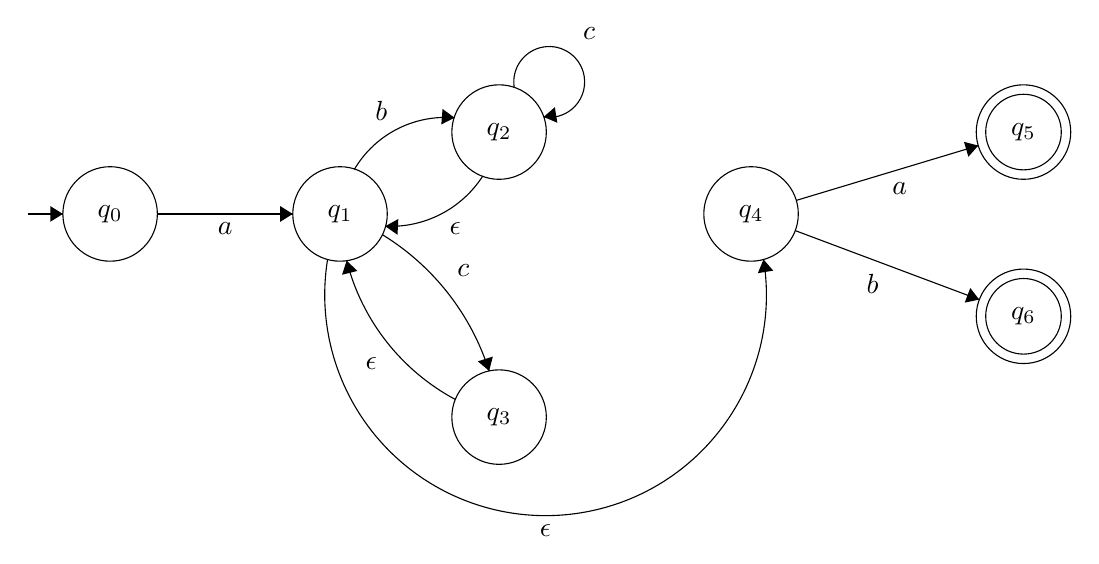
\begin{tikzpicture}[scale=0.2]
\tikzstyle{every node}+=[inner sep=0pt]
\draw [black] (9.8,-27) circle (3);
\draw (9.8,-27) node {$q_{0}$};
\draw [black] (24.4,-27) circle (3);
\draw (24.4,-27) node {$q_{1}$};
\draw [black] (34.5,-21.8) circle (3);
\draw (34.5,-21.8) node {$q_{2}$};
\draw [black] (34.5,-39.9) circle (3);
\draw (34.5,-39.9) node {$q_{3}$};
\draw [black] (50.5,-27) circle (3);
\draw (50.5,-27) node {$q_{4}$};
\draw [black] (67.8,-21.8) circle (3);
\draw (67.8,-21.8) node {$q_{5}$};
\draw [black] (67.8,-21.8) circle (2.4);
\draw [black] (67.8,-33.5) circle (3);
\draw (67.8,-33.5) node {$q_{6}$};
\draw [black] (67.8,-33.5) circle (2.4);
\draw [black] (4.6,-27) -- (6.8,-27);
\fill [black] (6.8,-27) -- (6,-26.5) -- (6,-27.5);
\draw [black] (12.8,-27) -- (21.4,-27);
\fill [black] (21.4,-27) -- (20.6,-26.5) -- (20.6,-27.5);
\draw (17.1,-27.5) node [below] {$a$};
\draw [black] (25.31,-24.167) arc (149.39749:85.08599:6.716);
\fill [black] (31.67,-20.89) -- (30.91,-20.33) -- (30.83,-21.32);
\draw (27.02,-21.11) node [above] {$b$};
\draw [black] (35.46,-18.97) arc (189:-99:2.25);
\draw (39.8,-15.55) node [right] {$c$};
\fill [black] (37.33,-20.84) -- (38.2,-21.21) -- (38.04,-20.22);
\draw [black] (33.464,-24.591) arc (-32.71907:-92.79744:6.955);
\fill [black] (27.27,-27.78) -- (28.05,-28.32) -- (28.1,-27.32);
\draw (31.71,-27.52) node [below] {$\epsilon$};
\draw [black] (27.091,-28.317) arc (58.47237:17.64566:15.758);
\fill [black] (33.87,-36.97) -- (34.1,-36.06) -- (33.15,-36.36);
\draw (31.82,-30.62) node [right] {$c$};
\draw [black] (31.723,-38.781) arc (-118.14883:-165.73314:13.877);
\fill [black] (24.82,-29.96) -- (24.53,-30.86) -- (25.5,-30.62);
\draw (26.78,-36.51) node [left] {$\epsilon$};
\draw [black] (51.293,-29.887) arc (9.22288:-189.22288:14.024);
\fill [black] (51.29,-29.89) -- (50.93,-30.76) -- (51.91,-30.6);
\draw (37.45,-46.66) node [below] {$\epsilon$};
\draw [black] (53.37,-26.14) -- (64.93,-22.66);
\fill [black] (64.93,-22.66) -- (64.02,-22.42) -- (64.3,-23.37);
\draw (59.94,-24.95) node [below] {$a$};
\draw [black] (53.31,-28.06) -- (64.99,-32.44);
\fill [black] (64.99,-32.44) -- (64.42,-31.7) -- (64.07,-32.63);
\draw (58.21,-30.77) node [below] {$b$};
\end{tikzpicture}

\noindent \textbf{\Large{QUIZ 5:}}\\
Let $\Sigma=\lbrace a,b \rbrace$, and given the language $L=$ All and only strings which do not include the substring $aaa$. Write a machine for $L$.\\


\noindent \textbf{\Large{Answer:}}\\


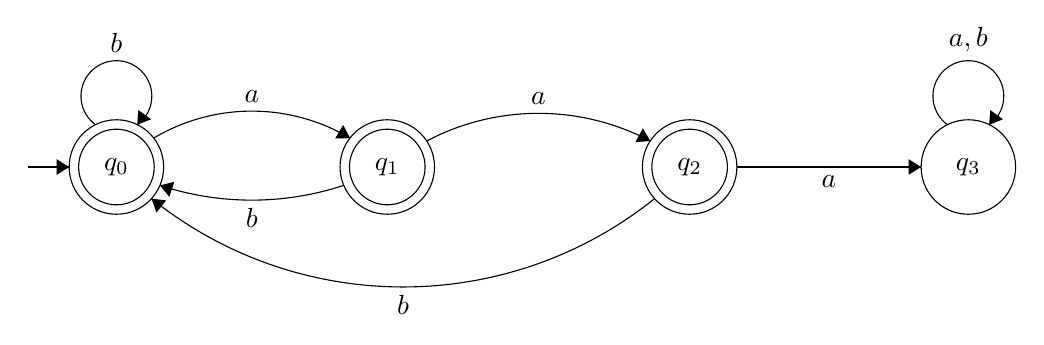
\begin{tikzpicture}[scale=0.2]
\tikzstyle{every node}+=[inner sep=0pt]
\draw [black] (11.6,-26.9) circle (3);
\draw (11.6,-26.9) node {$q_{0}$};
\draw [black] (11.6,-26.9) circle (2.4);
\draw [black] (28.8,-26.9) circle (3);
\draw (28.8,-26.9) node {$q_{1}$};
\draw [black] (28.8,-26.9) circle (2.4);
\draw [black] (48,-26.9) circle (3);
\draw (48,-26.9) node {$q_{2}$};
\draw [black] (48,-26.9) circle (2.4);
\draw [black] (65.7,-26.9) circle (3);
\draw (65.7,-26.9) node {$q_{3}$};
\draw [black] (6,-26.9) -- (8.6,-26.9);
\fill [black] (8.6,-26.9) -- (7.8,-26.4) -- (7.8,-27.4);
\draw [black] (13.964,-25.066) arc (120.75989:59.24011:12.193);
\fill [black] (26.44,-25.07) -- (26,-24.23) -- (25.49,-25.09);
\draw (20.2,-22.85) node [above] {$a$};
\draw [black] (31.299,-25.249) arc (117.80172:62.19828:15.224);
\fill [black] (45.5,-25.25) -- (45.03,-24.43) -- (44.56,-25.32);
\draw (38.4,-22.99) node [above] {$a$};
\draw [black] (51,-26.9) -- (62.7,-26.9);
\fill [black] (62.7,-26.9) -- (61.9,-26.4) -- (61.9,-27.4);
\draw (56.85,-27.4) node [below] {$a$};
\draw [black] (45.774,-28.909) arc (-51.30443:-128.69557:25.551);
\fill [black] (13.83,-28.91) -- (14.14,-29.8) -- (14.76,-29.02);
\draw (29.8,-35.02) node [below] {$b$};
\draw [black] (26.039,-28.065) arc (-71.72989:-108.27011:18.626);
\fill [black] (14.36,-28.07) -- (14.96,-28.79) -- (15.28,-27.84);
\draw (20.2,-29.5) node [below] {$b$};
\draw [black] (10.277,-24.22) arc (234:-54:2.25);
\draw (11.6,-19.65) node [above] {$b$};
\fill [black] (12.92,-24.22) -- (13.8,-23.87) -- (12.99,-23.28);
\draw [black] (64.377,-24.22) arc (234:-54:2.25);
\draw (65.7,-19.65) node [above] {$a,b$};
\fill [black] (67.02,-24.22) -- (67.9,-23.87) -- (67.09,-23.28);
\end{tikzpicture}
\clearpage


\section{Removing Non-Determinism}
\subsection{Non-Deterministic Finite Automata}
Let the NFA defined over the alphabet $\Sigma=\lbrace a, b \rbrace$.\\

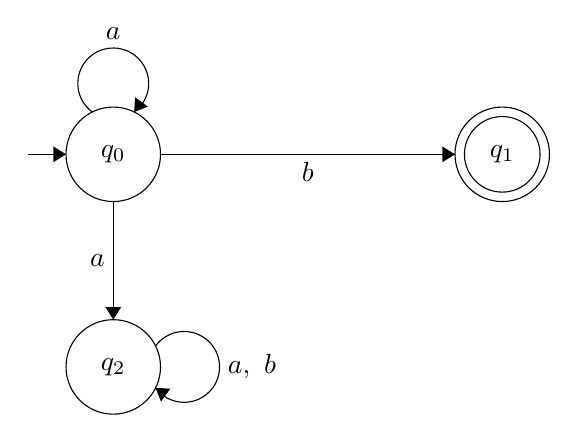
\begin{tikzpicture}[scale=0.2]
\tikzstyle{every node}+=[inner sep=0pt]
\draw [black] (19.6,-23.4) circle (3);
\draw (19.6,-23.4) node {$q_{0}$};
\draw [black] (44.3,-23.4) circle (3);
\draw (44.3,-23.4) node {$q_{1}$};
\draw [black] (44.3,-23.4) circle (2.4);
\draw [black] (19.6,-36.9) circle (3);
\draw (19.6,-36.9) node {$q_{2}$};
\draw [black] (22.6,-23.4) -- (41.3,-23.4);
\fill [black] (41.3,-23.4) -- (40.5,-22.9) -- (40.5,-23.9);
\draw (31.95,-23.9) node [below] {$b$};
\draw [black] (19.6,-26.4) -- (19.6,-33.9);
\fill [black] (19.6,-33.9) -- (20.1,-33.1) -- (19.1,-33.1);
\draw (19.1,-30.15) node [left] {$a$};
\draw [black] (18.277,-20.72) arc (234:-54:2.25);
\draw (19.6,-16.15) node [above] {$a$};
\fill [black] (20.92,-20.72) -- (21.8,-20.37) -- (20.99,-19.78);
\draw [black] (22.28,-35.577) arc (144:-144:2.25);
\draw (26.85,-36.9) node [right] {$a,\mbox{ }b$};
\fill [black] (22.28,-38.22) -- (22.63,-39.1) -- (23.22,-38.29);
\draw [black] (14.2,-23.4) -- (16.6,-23.4);
\fill [black] (16.6,-23.4) -- (15.8,-22.9) -- (15.8,-23.9);
\end{tikzpicture}

\begin{itemize}
\item The language of the NFA, $L(M)=$ $\lbrace$ x $\mid$ $(q_{0}, x)$ $\overset{*}{\vdash}$ $(q_{f}, \epsilon )\rbrace$
\item The grammar of the language, $L(G)=\lbrace $ $x$ $\mid$ $S\overset{*}{\Rightarrow}x\rbrace$
\item If your description is right and your machine is good, the sets of $L(M)$ and $L(G)$ will be equivalent.
\end{itemize}
\subsection{Removing non-determinism from finite-state computation}
\begin{itemize}
\item Let NFA, $M=\langle Q,\Sigma,\Delta, s,F \rangle$.
\item Define DFA, $M'=\langle Q',\Sigma,\delta, s',F' \rangle$.
\item Such that $L(M)=L(M')$
\end{itemize}

\underline{\textbf{Example}}\\
Let $\Sigma=\lbrace a,b\rbrace$ the alphabet of the language generated by the NFA, $M$ below.

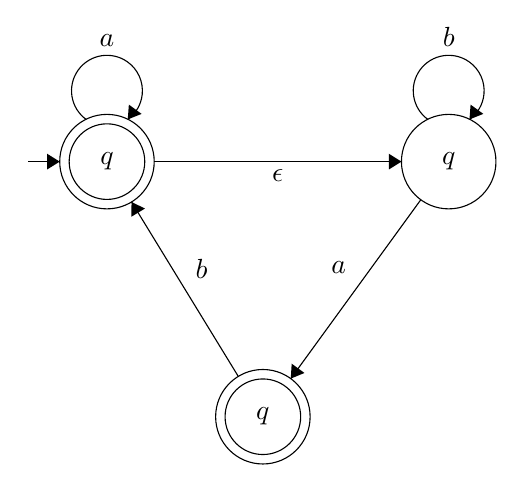
\begin{tikzpicture}[scale=0.2]
\tikzstyle{every node}+=[inner sep=0pt]
\draw [black] (16.5,-21.5) circle (3);
\draw (16.5,-21.5) node {$q$};
\draw [black] (16.5,-21.5) circle (2.4);
\draw [black] (38.2,-21.5) circle (3);
\draw (38.2,-21.5) node {$q$};
\draw [black] (26.4,-37.7) circle (3);
\draw (26.4,-37.7) node {$q$};
\draw [black] (26.4,-37.7) circle (2.4);
\draw [black] (15.177,-18.82) arc (234:-54:2.25);
\draw (16.5,-14.25) node [above] {$a$};
\fill [black] (17.82,-18.82) -- (18.7,-18.47) -- (17.89,-17.88);
\draw [black] (11.5,-21.5) -- (13.5,-21.5);
\fill [black] (13.5,-21.5) -- (12.7,-21) -- (12.7,-22);
\draw [black] (19.5,-21.5) -- (35.2,-21.5);
\fill [black] (35.2,-21.5) -- (34.4,-21) -- (34.4,-22);
\draw (27.35,-22) node [below] {$\epsilon$};
\draw [black] (36.877,-18.82) arc (234:-54:2.25);
\draw (38.2,-14.25) node [above] {$b$};
\fill [black] (39.52,-18.82) -- (40.4,-18.47) -- (39.59,-17.88);
\draw [black] (36.43,-23.92) -- (28.17,-35.28);
\fill [black] (28.17,-35.28) -- (29.04,-34.92) -- (28.23,-34.33);
\draw (31.72,-28.22) node [left] {$a$};
\draw [black] (24.84,-35.14) -- (18.06,-24.06);
\fill [black] (18.06,-24.06) -- (18.05,-25) -- (18.91,-24.48);
\draw (22.09,-28.32) node [right] {$b$};
\end{tikzpicture}

To eliminate the non-determinism, first what you need is $\epsilon-closure(q)=q\epsilon Q$. The closure of $\epsilon$ is all the states we can reach from $q$ by using $\epsilon -transitions$ only.

\begin{table}[H]
\begin{tabular}{|l|l|}
\hline
\multicolumn{2}{|c|}{$\epsilon -closure$}                              \\ \hline
\multicolumn{1}{|c|}{q0} & \multicolumn{1}{|c|}{\{$q_{0}$, $q_{1}$\}} \\ \hline
q1                       & \{$q_{1}$\}                          \\ \hline
q2                       & \{$q_{2}$\}                          \\ \hline
\end{tabular}
\end{table}

$s'=\epsilon -closure(s)$\\

$t=$ input transition function. $t(Q,a)=$ all the states we can go from $Q$ on $a$ before and after $\epsilon$-transition.

\begin{table}[H]
\begin{tabular}{c|cc}

$t$ & a              & b          \\ \hline
$q_{0}$ & \{$q_{0}$, $q_{1}$, $q_{2}$\} & \{$q_{1}$\}     \\ 
$q_{1}$ & \{$q_{2}$\}         & \{$q_{1}$\}     \\ 
$q_{2}$ & $\emptyset$           & \{$q_{0}$, $q_{1}$\} \\ 
\end{tabular}
\end{table}

The DFA, $M'$ of the NFA, $M$ above is shown below. The states of the machine are $Q_0$=$\left\lbrace q_0, q_1\right\rbrace$, $Q_1$=$\left\lbrace q_1\right\rbrace$, $Q_2$=$\left\lbrace q_2\right\rbrace$ and $Q_3$=$\left\lbrace q_0, q_1, q_2\right\rbrace$.\\

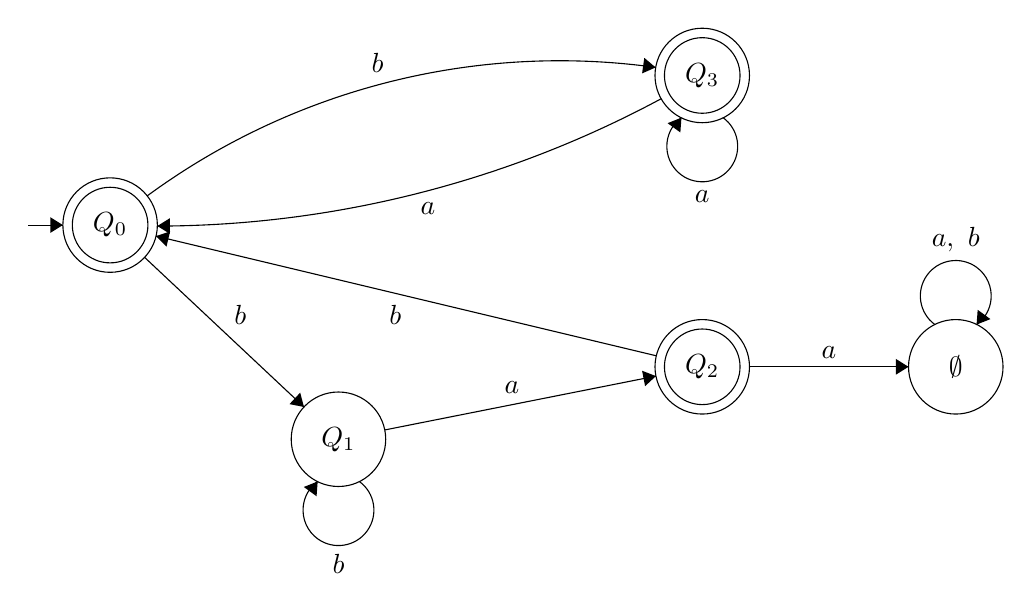
\begin{tikzpicture}[scale=0.2]
\tikzstyle{every node}+=[inner sep=0pt]
\draw [black] (14.1,-22) circle (3);
\draw (14.1,-22) node {$Q_0$};
\draw [black] (14.1,-22) circle (2.4);
\draw [black] (51.7,-12.5) circle (3);
\draw (51.7,-12.5) node {$Q_3$};
\draw [black] (51.7,-12.5) circle (2.4);
\draw [black] (28.6,-35.6) circle (3);
\draw (28.6,-35.6) node {$Q_1$};
\draw [black] (51.7,-31) circle (3);
\draw (51.7,-31) node {$Q_2$};
\draw [black] (51.7,-31) circle (2.4);
\draw [black] (67.8,-31) circle (3);
\draw (67.8,-31) node {$\emptyset$};
\draw [black] (8.9,-22) -- (11.1,-22);
\fill [black] (11.1,-22) -- (10.3,-21.5) -- (10.3,-22.5);
\draw [black] (16.457,-20.145) arc (126.27124:82.0879:44.275);
\fill [black] (48.74,-11.99) -- (48.02,-11.38) -- (47.88,-12.37);
\draw (31.08,-12.35) node [above] {$b$};
\draw [black] (49.09,-13.979) arc (-61.73101:-89.90985:67.772);
\fill [black] (17.1,-22.06) -- (17.9,-22.56) -- (17.9,-21.56);
\draw (34.28,-20.56) node [below] {$a$};
\draw [black] (16.29,-24.05) -- (26.41,-33.55);
\fill [black] (26.41,-33.55) -- (26.17,-32.64) -- (25.49,-33.37);
\draw (22.37,-28.32) node [above] {$b$};
\draw [black] (29.923,-38.28) arc (54:-234:2.25);
\draw (28.6,-42.85) node [below] {$b$};
\fill [black] (27.28,-38.28) -- (26.4,-38.63) -- (27.21,-39.22);
\draw [black] (31.54,-35.01) -- (48.76,-31.59);
\fill [black] (48.76,-31.59) -- (47.88,-31.25) -- (48.07,-32.23);
\draw (39.62,-32.72) node [above] {$a$};
\draw [black] (53.023,-15.18) arc (54:-234:2.25);
\draw (51.7,-19.75) node [below] {$a$};
\fill [black] (50.38,-15.18) -- (49.5,-15.53) -- (50.31,-16.12);
\draw [black] (54.7,-31) -- (64.8,-31);
\fill [black] (64.8,-31) -- (64,-30.5) -- (64,-31.5);
\draw (59.75,-30.5) node [above] {$a$};
\draw [black] (48.78,-30.3) -- (17.02,-22.7);
\fill [black] (17.02,-22.7) -- (17.68,-23.37) -- (17.91,-22.4);
\draw (32.21,-27.07) node [below] {$b$};
\draw [black] (66.477,-28.32) arc (234:-54:2.25);
\draw (67.8,-23.75) node [above] {$a,\mbox{ }b$};
\fill [black] (69.12,-28.32) -- (70,-27.97) -- (69.19,-27.38);
\end{tikzpicture}

$\delta(\left\lbrace q_0, q_1\right\rbrace a)$ = $t(q_0,a)$ $\cup$ $t(q_1,a)$\\

\indent \textit{\textbf{Quick Note:} When determining the final states of the DFA, the states which include final states of the NFA are selected. For example, in the NFA, $q_0$ and $q_2$ are the final states. Therefore, any state in the DFA which include these states are determined as the final states of the DFA.}\\

\noindent \textbf{\Large{QUIZ*:}}\\

*Because of the Covid-19 Pandemic, the lectures started to be conducted via online media. Therefore, the quiz at the end of the class was not given this week.

\section[Midterm Questions and Answers]{Midterm Questions and Answers\footnote{These questions do NOT reflect the real exam questions, and the answers are NOT the correct answers. They are all given just to provide a reference.}}

\textbf{Q1/4.} Consider the following finite automaton M1. Is it a DFA? In the simplest English description you can think of, what is the language of this machine?

$M_1 = (Q,\Sigma,\Delta,q_0,\lbrace q_0,q_1,q_2,q_3\rbrace)$ where $Q =\lbrace q_0,q_1,q_2,q_3,q_4\rbrace$ $\Sigma=\lbrace 0,1,2\rbrace $ and \\

$\Delta =\lbrace(q_0,0,q_1),(q_0,1,q_2),(q_0,2,q_3),(q_1,0,q_4),(q_1,1,q_2),(q_1,2,q_3),(q_2,0,q_1),$


$(q_2,1,q_4),(q_2,2,q_3),(q_3,0,q_1),(q_3,1,q_2),(q_3,2,q_4),(q_4,0,q_4),(q_4,1,q_4),(q_4,2,q_4)\rbrace$\\

\noindent \textbf{Q1/4.} The finite automaton $M_1$ is a DFA because each possible input determines the following state uniquely. In other words, the current state of the machine is changed by the input, and that input is totally responsible for determining that particular state. For example, if the machine $M_1$ is in the state $q_0$ and reads the input $1$, it goes to no other state but $q_2$. The same is valid for the other state-input combinations such as the fact that the combination $q_2$ and $2$ deterministically goes to $q_3$ and so on. Therefore, the machine $M_1$ is a DFA.\\
 
The language of this machine $L(M_1)$ is all and only the strings where no symbol occurs twice or more consecutively.

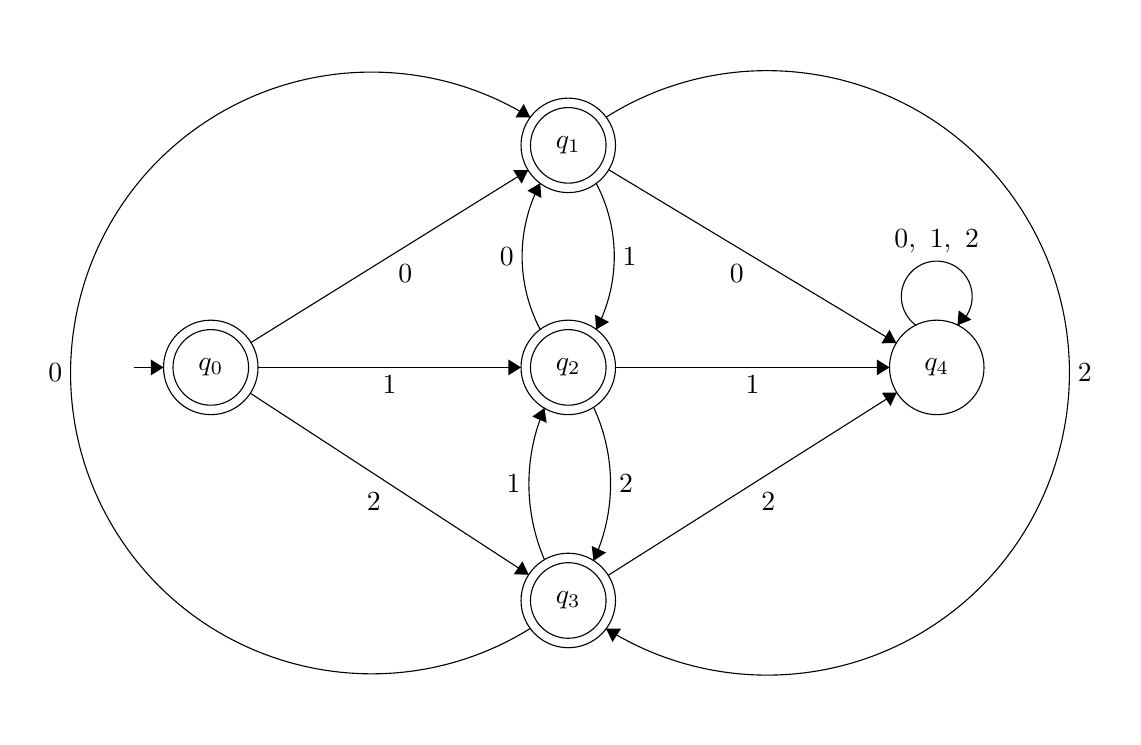
\begin{tikzpicture}[scale=0.2]
\tikzstyle{every node}+=[inner sep=0pt]
\draw [black] (14.7,-31.9) circle (3);
\draw (14.7,-31.9) node {$q_0$};
\draw [black] (14.7,-31.9) circle (2.4);
\draw [black] (37.4,-17.8) circle (3);
\draw (37.4,-17.8) node {$q_1$};
\draw [black] (37.4,-17.8) circle (2.4);
\draw [black] (37.4,-31.9) circle (3);
\draw (37.4,-31.9) node {$q_2$};
\draw [black] (37.4,-31.9) circle (2.4);
\draw [black] (37.4,-46.7) circle (3);
\draw (37.4,-46.7) node {$q_3$};
\draw [black] (37.4,-46.7) circle (2.4);
\draw [black] (60.8,-31.9) circle (3);
\draw (60.8,-31.9) node {$q_4$};
\draw [black] (9.8,-31.9) -- (11.7,-31.9);
\fill [black] (11.7,-31.9) -- (10.9,-31.4) -- (10.9,-32.4);
\draw [black] (17.25,-30.32) -- (34.85,-19.38);
\fill [black] (34.85,-19.38) -- (33.91,-19.38) -- (34.44,-20.23);
\draw (27.05,-25.35) node [below] {$0$};
\draw [black] (17.7,-31.9) -- (34.4,-31.9);
\fill [black] (34.4,-31.9) -- (33.6,-31.4) -- (33.6,-32.4);
\draw (26.05,-32.4) node [below] {$1$};
\draw [black] (17.21,-33.54) -- (34.89,-45.06);
\fill [black] (34.89,-45.06) -- (34.49,-44.21) -- (33.94,-45.04);
\draw (25.05,-39.8) node [below] {$2$};
\draw [black] (39.94,-45.1) -- (58.26,-33.5);
\fill [black] (58.26,-33.5) -- (57.32,-33.51) -- (57.86,-34.35);
\draw (50.1,-39.8) node [below] {$2$};
\draw [black] (40.4,-31.9) -- (57.8,-31.9);
\fill [black] (57.8,-31.9) -- (57,-31.4) -- (57,-32.4);
\draw (49.1,-32.4) node [below] {$1$};
\draw [black] (39.97,-19.35) -- (58.23,-30.35);
\fill [black] (58.23,-30.35) -- (57.8,-29.51) -- (57.29,-30.37);
\draw (48.1,-25.35) node [below] {$0$};
\draw [black] (39.173,-20.206) arc (27.77188:-27.77188:9.967);
\fill [black] (39.17,-29.49) -- (39.99,-29.02) -- (39.1,-28.55);
\draw (40.82,-24.85) node [right] {$1$};
\draw [black] (39.804,-16.01) arc (122.20156:-122.20156:19.192);
\fill [black] (39.8,-48.49) -- (40.21,-49.34) -- (40.75,-48.49);
\draw (69.72,-32.25) node [right] {$2$};
\draw [black] (35.622,-29.498) arc (-152.13044:-207.86956:9.943);
\fill [black] (35.62,-20.2) -- (34.81,-20.68) -- (35.69,-21.14);
\draw (33.97,-24.85) node [left] {$0$};
\draw [black] (39.005,-34.425) arc (24.99599:-24.99599:11.538);
\fill [black] (39,-44.18) -- (39.8,-43.66) -- (38.89,-43.24);
\draw (40.59,-39.3) node [right] {$2$};
\draw [black] (34.987,-48.477) arc (-58.13973:-301.86027:19.105);
\fill [black] (34.99,-16.02) -- (34.57,-15.18) -- (34.04,-16.03);
\draw (5.3,-32.25) node [left] {$0$};
\draw [black] (35.891,-44.116) arc (-156.75234:-203.24766:12.202);
\fill [black] (35.89,-34.48) -- (35.12,-35.02) -- (36.03,-35.42);
\draw (34.4,-39.3) node [left] {$1$};
\draw [black] (59.477,-29.22) arc (234:-54:2.25);
\draw (60.8,-24.65) node [above] {$0,\mbox{ }1,\mbox{ }2$};
\fill [black] (62.12,-29.22) -- (63,-28.87) -- (62.19,-28.28);
\end{tikzpicture}

\noindent \textbf{Q2/4.} Now try to express the language above formally. In other words, write a regular expression for $L(M_1)$.\\

\noindent \textbf{Q2/4.}\\

$\Big($0(1 $|$ 2) $|$ 0( $(12)^{+}$(1 $|$ $\epsilon$) $|$ $(21)^{+}$(2 $|$ $\epsilon$) )$\Big)^{*}$ $\Big($0 $|$ $\epsilon \Big)$ $\Big|$ 

$\Big($1(0 $|$ 2) $|$ 1( $(02)^{+}$(0 $|$ $\epsilon$) $|$ $(20)^{+}$(2 $|$ $\epsilon$) )$\Big)^{*}$ $\Big($1 $|$ $\epsilon \Big)$ $\Big|$

$\Big($2(0 $|$ 1) $|$ 2( $(10)^{+}$(1 $|$ $\epsilon$) $|$ $(01)^{+}$(0 $|$ $\epsilon$) )$\Big)^{*}$ $\Big($2 $|$ $\epsilon \Big)$

\clearpage

\noindent \textbf{Q3/4.} Eliminate non-determinism from the following NFA $M_3 =(\lbrace q_0,q_1\rbrace,\lbrace 0,1\rbrace ,\Delta_3,q0,\lbrace q_0\rbrace)$ where $\Delta_{3} =\lbrace(q_0,0,q_0),(q_0,0,q_1),(q_0,1,q_0),(q_0,1,q_1),(q_1,1,q_1)\rbrace.$\\

\noindent \textbf{Q3/4.}\\
\indent \textit{The NFA:}\\

\noindent
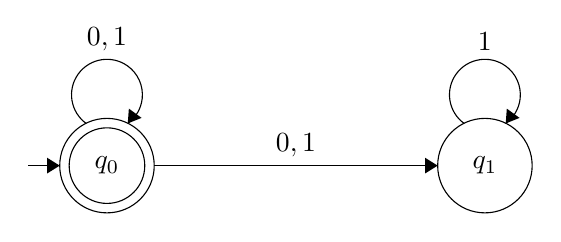
\begin{tikzpicture}[scale=0.2]
\tikzstyle{every node}+=[inner sep=0pt]
\draw [black] (16,-30.8) circle (3);
\draw (16,-30.8) node {$q_0$};
\draw [black] (16,-30.8) circle (2.4);
\draw [black] (40,-30.8) circle (3);
\draw (40,-30.8) node {$q_1$};
\draw [black] (11,-30.8) -- (13,-30.8);
\fill [black] (13,-30.8) -- (12.2,-30.3) -- (12.2,-31.3);
\draw [black] (19,-30.8) -- (37,-30.8);
\fill [black] (37,-30.8) -- (36.2,-30.3) -- (36.2,-31.3);
\draw (28,-30.3) node [above] {$0,1$};
\draw [black] (14.677,-28.12) arc (234:-54:2.25);
\draw (16,-23.55) node [above] {$0,1$};
\fill [black] (17.32,-28.12) -- (18.2,-27.77) -- (17.39,-27.18);
\draw [black] (38.677,-28.12) arc (234:-54:2.25);
\draw (40,-23.55) node [above] {$1$};
\fill [black] (41.32,-28.12) -- (42.2,-27.77) -- (41.39,-27.18);
\end{tikzpicture}

$\epsilon$-closure states: I assumed that by using $\epsilon$ we can only stay in the current state, although $\epsilon$-transitions are not explicitly stated; actually there is none. Therefore, I have left the table anyway. 
\begin{table}[H]
\begin{tabular}{|c|c|}
\hline
     & $\epsilon$ \\ \hline
$q_0$ & \{$q_0$\}  \\ \hline
$q_1$ & \{$q_1$\}  \\ \hline
\end{tabular}
\end{table}


Input transition function \emph{(t)}:
\begin{table}[H]
\begin{tabular}{|c|c|c|}
\hline
$t$     & 0              & 1      \\ \hline
$q_0$ & \{$q_0, q_1$\} & \{$q_0, q_1$\} \\ \hline
$q_1$ & $\emptyset$    & \{$q_1$\} \\ \hline
\end{tabular}
\end{table}


\emph{The DFA, $M_3^{'}$ of the NFA, $M_3$:}\\

\noindent
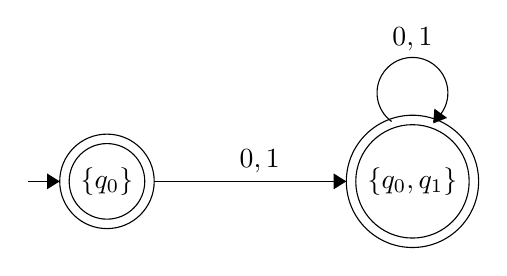
\begin{tikzpicture}[scale=0.2]
\tikzstyle{every node}+=[inner sep=0pt]
\draw [black] (15.8,-30.8) circle (3);
\draw (15.8,-30.8) node {$\{q_0\}$};
\draw [black] (15.8,-30.8) circle (2.4);
\draw [black] (35.2,-30.8) circle (4.2);
\draw (35.2,-30.8) node {$\{q_0,q_1\}$};
\draw [black] (35.2,-30.8) circle (3.6);
\draw [black] (10.8,-30.8) -- (12.8,-30.8);
\fill [black] (12.8,-30.8) -- (12,-30.3) -- (12,-31.3);
\draw [black] (18.8,-30.8) -- (31,-30.8);
\fill [black] (31,-30.8) -- (30.2,-30.3) -- (30.2,-31.3);
\draw (25.5,-30.3) node [above] {$0,1$};
\draw [black] (33.877,-27) arc (234:-54:2.25);
\draw (35.2,-22.55) node [above] {$0,1$};
\fill [black] (36.52,-27.12) -- (37.4,-26.77) -- (36.59,-26.18);
\end{tikzpicture}

$M_3^{'}$=($\lbrace \lbrace q_0\rbrace,\lbrace q_0,q_1\rbrace\rbrace ,\lbrace 0,1\rbrace ,\delta_{3}, \lbrace q_0 \rbrace , \lbrace \lbrace q_0\rbrace,\lbrace q_0,q_1\rbrace\rbrace$) where


$\delta_{3}=\lbrace (\lbrace q_0\rbrace ,0,\lbrace q_0,q_1\rbrace),(\lbrace q_0\rbrace ,1,\lbrace q_0,q_1\rbrace), (\lbrace q_0,q_1\rbrace, 0,\lbrace q_0,q_1\rbrace),(\lbrace q_0,q_1\rbrace, 1,\lbrace q_0,q_1\rbrace)\rbrace$

\clearpage

\noindent \textbf{Q4/4.} The grammar below captures a small fragment of our arithmetic, of addition and multiplication of single-digit numbers. For example, 5+(3x2) is well-formed, whereas 5+x(32) is not.\\


$S \rightarrow S+T$ $|$ $T$\\
\indent $T \rightarrow T+F$ $|$ $F$\\
\indent $F \rightarrow 0|1|\cdots |9|(S)$\\

First, draw a tree for the well-formed example above using this grammar.\\ Second, it seems that it captures more than just well-formedness of these simple arithmetic expressions. To see this, compare the following grammar for the same language: \\

$S_2 \rightarrow S_2 + S_2 |S_2 x S_2 |0|1|\cdots|9|(S_2)$\\

What is the property that grammar of (1-3) captures and (4) does not? Would you call this a semantic property, structural, both, or what?\\

\noindent \textbf{Q4/4.}\\

\begin{tikzpicture}
\draw (0,0) -- (1.5,0.50) -- (3,0);
\node at (1.5,0.75) {S};
\node at (0,-0.25) {S};
\draw (0,-0.5) -- (0,-1);
\node at (0,-1.25) {T};
\draw (0,-1.5) -- (0,-2);
\node at (0,-2.25) {F};
\node at (0,-2.75) {5};
\draw (1.5,0.5) -- (1.5,-0.25);
\node at (1.5,-0.5) {+};
\draw (1.5,-1) -- (3,-0.5) -- (4.5,-1);
\node at (3,-0.25) {T};
\node at (1.5,-1.25) {T};
\draw (1.5,-1.5) -- (1.5,-2);
\node at (1.5,-2.25) {F};
\node at (1.5,-2.75) {3};
\node at (4.5,-1.25) {F};
\node at (4.5,-1.75) {2};
\draw (3,-0.5) -- (3,-1);
\node at (3,-1.25) {x};
\end{tikzpicture}
\\

Unlike the first one, the second grammar cannot differentiate \emph{the order of the operations} ($+$ and $x$), which creates an ambiguity in that the grammar accepts not only $5+(3x2)$ but also $(5+3)x2$ without parentheses, seeing the trees below. I would call this as a structural ambiguity which has a semantic implication because this ambiguous structure causes different end results; that is, the meaning of the strings are not the same although they have the same order. Therefore, the property of the first grammar is both structural and semantic.\\ 


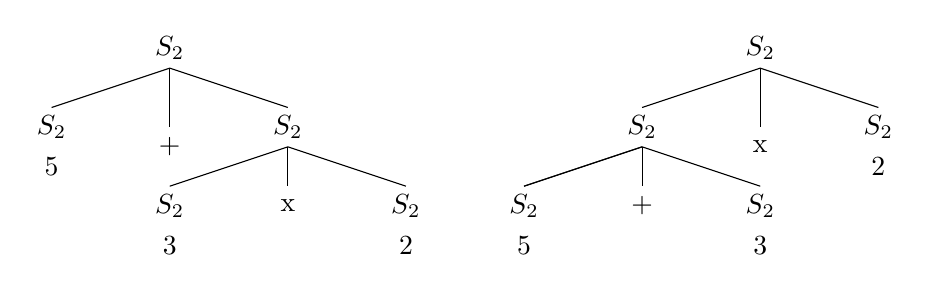
\begin{tikzpicture}
\draw (0,0) -- (1.5,0.50) -- (3,0);
\node at (1.5,0.75) {$S_2$};
\node at (0,-0.25) {$S_2$};
\node at (0,-0.75) {5};
\draw (1.5,0.5) -- (1.5,-0.25);
\node at (1.5,-0.5) {+};
\draw (1.5,-1) -- (3,-0.5) -- (4.5,-1);
\node at (3,-0.25) {$S_2$};
\node at (1.5,-1.25) {$S_2$};
\node at (1.5,-1.75) {3};
\node at (4.5,-1.25) {$S_2$};
\node at (4.5,-1.75) {2};
\draw (3,-0.5) -- (3,-1);
\node at (3,-1.25) {x};

\draw (7.5,0) -- (9,0.50) -- (10.5,0);
\node at (9,0.75) {$S_2$};
\node at (7.5,-0.25) {$S_2$};
\draw (7.5,-0.5) -- (6,-1);
\node at (7.5,-1.25) {+};
\draw (9,0.5) -- (9,-0.25);
\node at (9,-0.5) {x};
\node at (10.5,-0.25) {$S_2$};
\node at (6,-1.25) {$S_2$};
\node at (6,-1.75) {5};
\draw (6,-1) -- (7.5,-0.5) -- (9,-1);
\node at (9,-1.25) {$S_2$};
\node at (9,-1.75) {3};
\node at (10.5,-0.75) {2};
\draw (7.5,-0.5) -- (7.5,-1);

\end{tikzpicture}

\clearpage

\section{Lambda Calculus}
Lambda Calculus, coined by \textbf{Alonzo Church} is a glue language for syntax-semantics connection and a theory of substitution. According to \textbf{Frege's Principle of Compositionality}, the meaning of the whole is a function of the meaning of the parts and the way they are combined. Emmon Bach's Rule-to-Rule Thesis (1976) stated that a semantic rule accompanies the application of a syntactic rule. Semantic rules are functions and arguments.


\subsection{Conversions in $\lambda$-Calculus}
There is a set of conversions in $\lambda$-calculus. Conversion means any abstraction or reduction.

\begin{itemize}
\item \textbf{$\lambda$ conversion}
\item \textbf{$\beta$ conversion:} $(\lambda x.M]N=\beta M[N/x]$ (substitution of $N$ for free occurrences of $x$ in $M$)\emph{ e.g.:} $(\lambda x.-x$ $2)3=\beta (-x$ $2)[3/x]=(-3$ $2)=1$
\item \textbf{$\alpha$ conversion}
\item \textbf{$\eta$ conversion}
\end{itemize}

\subsection{$\lambda$-terms}
There are some $\lambda$-terms.

\begin{itemize}
\item \textbf{Constants} \textit{(0, 1, John, ...)}
\item \textbf{Variables} \textit{(x, y, $x_1$, ...)}
\item If $M$ is a $\lambda$-term, and $x$ is a variable, then $\lambda x.M$ is a $\lambda$-term.
\item If $M$ and $N$ are $\lambda$-terms, $MN$ is also a $\lambda$-term.
\end{itemize} 

\textit{\textbf{Quick Note: }Arguments themselves can be functions as well.}\\

$\lambda x.x^{2}$ applies square function. $(\lambda x.x2)sqr=(x$ $2)[sqr/x]=sqr$ 2\\

\noindent $sqr=\lambda y.x$ $yy$, $(\lambda z. zz)(\lambda y. x$ $yy)=\beta (z$ $z)[(\lambda y.x$ $yy)/z]=(\lambda y.x$ $yy)z=\beta (x$ $yy)[z/y]=(x$ $zz)$\\

\textit{\textbf{Quick Note: }Form-meaning correspondence can be implemented by $\lambda$-calculus.}\\

\subsection{Beta-Reducible Expression ($\beta$-Redex)}
A $\lambda$-term is a $\beta$-redex if it is of the form $(\lambda x.M)N$ which can be reduced to the form $M[N/x]$.\\

Here is the problem. What if there is more than one $\beta$-redex? Which one is evaluated first?. There are two kinds of order of evaluation:
\begin{enumerate}
\item Normal Order of Evaluation (NOE): Evaluate outermost and leftmost $\beta$-redex first.
\item Applicative Order of Evaluation (AOE): Evaluate the innermost leftmost $\beta$-redex first.
\end{enumerate}

\textbf{Church-Russer Theorem of Property:} If a $\lambda$-term has a normal form (a form which is not further reducible), then NOE and AOE give the same normal order.\\

Take the following $\lambda$-term $(\lambda g.\lambda x. gx)((\lambda y.+$ $y$ 2) 3)\\

By AOE, we get $(\lambda x.((\lambda y.+$ $y$ 2) 3) x)= $\lambda x.$(+ 3 2) \textit{x}\\

By NOE, we get $(\lambda g.gx)(+$ 3 2)= $\lambda x.$(+ 3 2) \textit{x}\\

Some $\lambda$-terms have no normal form. e.g.: $(\lambda x.xx)(\lambda y.yy)$ $=_\beta$ $(\lambda y.yy)(\lambda y.yy)$ when this expression $\beta$-reduced again, the result will be the same, so there is an endless loop here.

\subsection{Formal Capture of Structure in Cognition}

\begin{itemize}
\item Syntax (form) $\rightarrow$ Automata, CFG
\item Semantics (meaning) $\rightarrow$ Lambda Calculus
\item Uncertainty (inference) $\rightarrow$ Probability, Parsing
\end{itemize}

\textbf{The combination of Syntax and Semantics in Mini-English}\\

$S:\lambda x \lambda y.yx\rightarrow$ $NP:np^{'}$ $VP:vp^{'}$\\
\indent $VP:\lambda x \lambda y.xy\rightarrow$ $V_{T}:v^{'}$ $NP:np^{'}$\\
\indent $VP:\lambda x \lambda y.xy\rightarrow$ $V_{C}:v^{'}$ $S:s^{'}$\\
\indent $V_{T}:\lambda x.x\rightarrow$ $like:\lambda x \lambda y$ $like^{'}$ $xy$\\
\indent $V_{C}:\lambda x.x\rightarrow$ $think:\lambda x \lambda y$ $think^{'}$ $xy$\\


\clearpage

\noindent \textbf{\Large{QUIZ 6:}}\\
Consider the following lambda term, $(\lambda g.\lambda x.gx)(\lambda y.-$ 2 $y)(3)$\\

\textbf{Q1.} Write the lambda term in tree notation.\\
\indent \textbf{Q2.} Evaluate the lambda term using beta-reduction.\\

\noindent \textbf{\Large{Answer:}}\\

\textbf{Question 1:}\\

\begin{tikzpicture}
\draw (0,0) -- (1.5,0.50) -- (3,0);
\node at (1.5,0.75) {$\lambda$};
\node at (0,-0.25) {$g$};
\draw (1.5,-1) -- (3,-0.5) -- (4.5,-1);
\node at (3,-0.25) {$\lambda$};
\node at (1.5,-1.25) {$x$};
\draw (3,-2) -- (4.5,-1.5) -- (6,-2);
\node at (4.5,-1.25) {$gx$};
\draw (6,-2.5) -- (6,-3);
\node at (6,-3.25) {3};
\node at (3,-2.25) {$g$};
\draw (3,-2.5) -- (3,-3);
\node at (3,-3.25) {$\lambda$};
\draw (1.5,-4) -- (3,-3.5) -- (4.5,-4);
\node at (6,-2.25) {x};
\node at (1.5,-4.25) {$y$};
\node at (4.5,-4.25) {$app$};
\draw (3,-5) -- (4.5,-4.5) -- (6,-5);
\node at (3,-5.25) {$app$};
\node at (6,-5.25) {$y$};
\draw (1.5,-6) -- (3,-5.5) -- (4.5,-6);
\node at (1.5,-6.25) {$-$};
\node at (4.5,-6.25) {2};
\end{tikzpicture}
\\

\noindent \textbf{Question 2:}\\
\noindent $(\lambda g.\lambda x.gx)(\lambda y.-$ 2 $y)(3)$\\
$=_{\beta}((\lambda x.gx)[(\lambda y.-$ 2 $y)/g])(3)$\\
$=(\lambda x.(\lambda y.-$ 2 $y)x)(3)$\\
$=_{\beta}((\lambda y.-$ 2 $y)x)[3/x]$\\
$=(\lambda y.-$ 2 $y)(3)$\\
$=_{\beta}(-$ 2 $y)[3/y]$\\
$=-$ 2 3\\
$=(-1)$\\

\clearpage

\noindent \textbf{\Large{QUIZ 7:}}\\
Let's take the following lambda term, $((\lambda f.f$ 4)($\lambda h.h$ 2))}(($\lambda g.g$ 3) +)

\begin{enumerate}
\item Reduce the term using Normal Order Evaluation.
\item Reduce the term using Applicative Order Evaluation.
\end{enumerate}



\noindent \textbf{\Large{Answer:}}\\

\noindent \textbf{Normal Order Evaluation:\footnote{Leftmost outermost $\beta$-redexes are underlined.}} \\
\underline{$((\lambda f.f$ 4)($\lambda h.h$ 2))}(($\lambda g.g$ 3) +)\\
=\underline{(($\lambda h.h$ 2) 4)(($\lambda g.g$ 3) +)}\\
=(((\underline{($\lambda g.g$ 3) +)} 2) 4)\\
=(((+ 3) 2) 4)\\

\noindent \textbf{Applicative Order Evaluation:\footnote{Leftmost innermost $\beta$-redexes are underlined.}}\\
\underline{$((\lambda f.f$ 4)($\lambda h.h$ 2))}(($\lambda g.g$ 3) +)\\
=(($\lambda h.h$ 2) 4)\underline{(($\lambda g.g$ 3) +)}\\
=\underline{(($\lambda h.h$ 2) 4)(+ 3)}\\
=(((+ 3) 2) 4)\\
\clearpage

\section{Push Down Automata (PDA)}
PDA is a finite state machine with a stack. PDA, $M=(Q,\Sigma,\Gamma,\Delta,s,F)$ where $\Gamma$ includes the stack symbols, the rest is the same as those of an FSA.\\

\textbf{Configuration of a PDA:} (current state, remainder of input, current content of the stack)\\

\textbf{Elements of $\Delta$:} $((p,a,A),(q,B))$ where $p$ is the current state, $a$ is the current symbol, $A$ is the top of stack, $q$ is the next state and $B$ is the new top of the stack.\\

In current state $p$ , scan $a$, pop $A$, go to $q$, push $B$; where $p,q\in Q$, $a\in \Sigma^{*} \cup \lbrace \epsilon \rbrace$, $A,B \in \Gamma^{*} \cup \lbrace \epsilon \rbrace$\\

\underline{\textbf{Example:}} $L=\lbrace a^{n}b^{n}|n\geq0\rbrace$\\

$G(L)= S\rightarrow aSb|\epsilon$\\

\textbf{Ad hoc PDA construction:}\\

$\Delta= ((p,a,\epsilon),(p,A99,((p,b,A),(q,\epsilon)),((q,b,A),(q,\epsilon))$\\
 
$L(M)=\lbrace w\in \Sigma^{*}|(s,w,\epsilon)\vdash^{*}(p,\epsilon,\epsilon), p\in F\rbrace$\\

\subsection{Algorithm for PDA Construction from CFG}
Let CFG $G=(V,\Sigma,R,S)$ where all rules in $R$ are $\alpha \rightarrow \beta$, $\alpha \in V$ and $\beta \in (V\cup\Sigma)^*$\\

Define PDA, $M=(\lbrace p, g\rbrace,\Sigma, V\cup \Sigma,\Delta,p,\lbrace q\rbrace)$\\

For every $\alpha \rightarrow \beta$ in R,\\
Define $((p,\epsilon,\beta^R),(p,\alpha))$ in $\Delta$\\

For every $a \in \Sigma$,\\ 
Define $((p,a,\epsilon),(p,a))$ in $\Delta$\\
Define $((p,\epsilon,S),(q,\epsilon))$, then $L(G)=L(M)$\\

\clearpage

\noindent \textbf{\Large{QUIZ 8:}}\\
Let us take a small fragment of arithmetic grammar, this time using
semantic rules as well.\\

\noindent $S:\lambda x.\lambda y.\lambda z. yxz \rightarrow S:s^{'}$ $+:+$ $T:t^{'}$\\
$S:\lambda x.x \rightarrow T:t^{'}$\\
$T:\lambda x.x \rightarrow F:f^{'}$\\
$F:\lambda x.x \rightarrow$ 3:3 $|$ 5:5\\

\begin{enumerate}
\item Construct the PDA using the algorithm.
\item Compute the result of 3+5 using the PDA. Show use of syntactic rule and semantic action where appropriate.
\end{enumerate}

\noindent \textbf{\Large{Answer:}}\\
\textbf{Question 1:}\\
$((p,3,\epsilon),(p,3))$\\
$((p,5,\epsilon),(p,5))$\\
$((p,+,s^{'}),(p,+))$\\
$((p,\epsilon,3),(p,F:(\lambda x.x)3=f^{'}))$\\
$((p,\epsilon,5),(p,F:(\lambda x.x)5=f^{'}))$\\
$((p,\epsilon,F),(p,T:(\lambda x.x)f^{'})=t^{'})$\\
$((p,\epsilon,T),(p,S:(\lambda x.x)t^{'})=s^{'})$\\
$((p,\epsilon,t^{'}+s^{'}),(p,S:((\lambda x.\lambda y.\lambda z. yxz)s^{'}+t^{'})))$\\
$((p,\epsilon,S),(q,\epsilon))$\\

\noindent \textbf{Question 2:}\\
$(p,3+5,\epsilon)\vdash$\\
$(p,+5,3)\vdash$\\
$(p,+5,F:(\lambda x.x)3)\vdash$\\
$(p,+5,T:(\lambda x.x)f^{'})\vdash$\\
$(p,+5,S:(\lambda x.x)t^{'})\vdash$\\
$(p,+5,s^{'})\vdash$\\
$(p,5,+s^{'})\vdash$\\
$(p,\epsilon, (F:(\lambda x.x)5)+s^{'})\vdash$\\
$(p,\epsilon, (T:(\lambda x.x)f^{'})+s^{'})\vdash$\\
$(p,\epsilon,t^{'}+s^{'})\vdash$\\
$(p,\epsilon,S:((\lambda x.\lambda y.\lambda z. yxz)t^{'}+s^{'}))\vdash$\\
$(p,\epsilon,S)\vdash$\\
$(q,\epsilon)$ and accept.

\clearpage

\section{Computational Uncertainty}
\noindent \textbf{\Large{QUIZ 9:}}\\
In Part 2 of week 13 video, from 6:24 to 8:44 I show a joint distribution of a sentence and tree as product of probabilities of rule use. If you look at how I conditionalize the probabilities, you will see that it assumes that the tree is built bottom-up.\\

\noindent \textbf{Question 1:} Comment on why this is the case.\\
\noindent \textbf{Question 2:} If the tree is to be built top-down, what would the joint distribution be, in terms of product of conditional probabilities?\\

\noindent \textbf{\Large{Answer:}}\\

\noindent \textbf{Question 1:} The tree is built bottom-up because the units that constitute the sentence such as NP, VP and PP are assumed to form the sentence, and they are assumed to be formed by other units such as $V$ and $P_{with}$ etc. Therefore, if the tree was built in top-down fashion, the joint probability of the tree would be determined by the surface items such as \textit{I, saw, telescope, the etc.} given the sentence $S$ and the phrase they constitute. Therefore, the joint probability of the sentence would be calculated from these surface items if the tree were built in top-down assumption. Although the build-architectures are different, this will not affect the joint probability (but I cannot be sure as we do not have any value indicating the probability values of the phrases and surface items).\\

\noindent \textbf{Question 2:} $P(T|S)=P(S|I)\times P(NP|I)\times P(S|saw)\times P(VP_{1}|saw)\times P(VP_{2}|saw)\times P(V|saw)\times P(S|the$ $man)\times P(VP_{1}|the$ $man)\times P(VP_{2}|the$ $man)\times P(NP|the$ $man)\times P(P_{with}|with)\times P(PP|with)\times P(VP_{1}|with)\times P(S|with)\times P(NP|the$ $telescope)\times P(PP|the$ $telescope)\times P(VP_{1}|the$ $telescope)\times P(S|the$ $telescope)$

\clearpage

\section{Final Exam Questions and Answers}
\textbf{QUESTIONS:}\\

\noindent We are given a language of the sequence of the symbol `$ \bigtriangleup $' separating two single-digit natural numbers. In the general form the input is $n$ is $n\bigtriangleup \cdots \bigtriangleup m $. It means $(((n^{2})^{2})\cdots^{2})-m$, where the number of squaring is the number of occurrences of $\bigtriangleup$ in the sequence. For example, $5\bigtriangleup\bigtriangleup3$ means 625-3 because $((5^{2})^{2})-3=625-3$, and $2\bigtriangleup\bigtriangleup\bigtriangleup4$ means $256-4$. The sequence $5$ $3$ means $5-3$. We would expect the following trees for these examples:\\

\hspace{1cm}
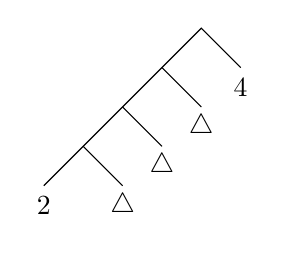
\begin{tikzpicture}
\draw (-2,-2) -- (0,0) -- (0.5,-0.5);
\draw (-1.5,-1.5) -- (-1,-2);
\draw (-1,-1) -- (-0.5,-1.5);
\draw (-0.5,-0.5) -- (0,-1);
\node at (-2,-2.25) {$2$};
\node at (-1,-2.25) {$\bigtriangleup$};
\node at (-0.5,-1.75) {$\bigtriangleup$};
\node at (0,-1.25) {$\bigtriangleup$};
\node at (0.5,-0.75) {$4$};
\end{tikzpicture}
\hspace{2cm}
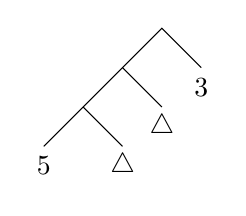
\begin{tikzpicture}
\draw (-1.5,-1.5) -- (0,0) -- (0.5,-0.5);
\draw (-1,-1) -- (-0.5,-1.5);
\draw (-0.5,-0.5) -- (0,-1);
\node at (-1.5,-1.75) {$5$};
\node at (-0.5,-1.75) {$\bigtriangleup$};
\node at (0,-1.25) {$\bigtriangleup$};
\node at (0.5,-0.75) {$3$};
\end{tikzpicture}
\hspace{2cm}
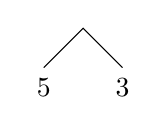
\begin{tikzpicture}
\draw (-0.5,-0.5) -- (0,0) -- (0.5,-0.5);
\node at (-0.5,-0.75) {$5$};
\node at (0.5,-0.75) {$3$};
\end{tikzpicture}

\noindent The following grammar can generate these trees once we treat `$\bigtriangleup$' as the square function:\\

$S\rightarrow AN$ where $N$ is a natural number between 0 and 9.\\	
\indent $A\rightarrow A\bigtriangleup$\\
\indent $A\rightarrow N$\\

\begin{enumerate}
\item (10 points) If we were only interested in the form, this would be a regular language. Write a regular expression for it.
\item (20 points) Since we are not only interested in form in this course, we should be able to interpret the trees above from grammar. Show how the first tree above can be evaluated step by step, using lambda terms in the process.
\item  (30 points) Show a PDA that does form-meaning computation for this language in locked-step with rule use.
\item (40 points) Since we are not only interested in this course about the form, its meaning and locked-step computation of its structure, but also about how they behave altogether under uncertainty, we might want to look into some models of this phenomenon in extended use.\\
Suppose that the owner/processor of this system notices that what she can do with squaring she can also do with self-addition (symbolized by $\ddagger$) to get the same result, or a mixture of the two. For example:
\end{enumerate}
\hspace{3cm}
\begin{tikzpicture}
\draw (-2,-2) -- (0,0) -- (0.5,-0.5);
\draw (-1.5,-1.5) -- (-1,-2);
\draw (-1,-1) -- (-0.5,-1.5);
\draw (-0.5,-0.5) -- (0,-1);
\node at (-2,-2.25) {$3$};
\node at (-1,-2.25) {$\ddagger$};
\node at (-0.5,-1.75) {$\bigtriangleup$};
\node at (0,-1.25) {$\ddagger$};
\node at (0.5,-0.75) {$2$};
\node at (1.5,-0.5) {$=70$};
\node at (3,-0.5) {and};
\end{tikzpicture}
\begin{tikzpicture}
\draw (-2,-2) -- (0,0) -- (0.5,-0.5);
\draw (-1.5,-1.5) -- (-1,-2);
\draw (-1,-1) -- (-0.5,-1.5);
\draw (-0.5,-0.5) -- (0,-1);
\draw (-2.5,-2.5) -- (-2,-2) -- (-1.5,-2.5);
\node at (-2.5,-2.75) {$3$};
\node at (-1.5,-2.75) {$\bigtriangleup$};
\node at (-1,-2.25) {$\ddagger$};
\node at (-0.5,-1.75) {$\ddagger$};
\node at (0,-1.25) {$\ddagger$};
\node at (0.5,-0.75) {$2$};
\node at (1.5,-0.5) {$=70$};
\end{tikzpicture}
\clearpage

\noindent \textbf{ANSWERS\footnote{These questions do NOT reflect the real exam questions, and the answers are NOT the correct answers. They are all given just to provide a reference.}:}\\
\noindent \textbf{Question 1:} $(0|1|2|3|4|5|6|7|8|9)$ $ \bigtriangleup^{*} $ $(0|1|2|3|4|5|6|7|8|9)$\\ where $\bigtriangleup$ corresponds to 2 that squares its argument.\\

\noindent \textbf{Question 2:}\\
$=(\lambda f. \lambda g (-$ $f$ $g$))$((\lambda x. \lambda y.x^{y})((\lambda z. \lambda w.z^{w})(5\bigtriangleup \bigtriangleup 3)))$\\
$=_{\beta}(\lambda f. \lambda g (-$ $f$ $g$))$((\lambda x. \lambda y.x^{y})((\lambda z. \lambda w.z^{w})[5/z](\bigtriangleup \bigtriangleup 3)))$\\
$=(\lambda f. \lambda g (-$ $f$ $g$))$((\lambda x. \lambda y.x^{y})((\lambda w.5^{w})(\bigtriangleup \bigtriangleup 3)))$\\
$=_{\beta}(\lambda f. \lambda g (-$ $f$ $g$))$((\lambda x. \lambda y.x^{y})((\lambda w.5^{w}[\bigtriangleup/w](\bigtriangleup 3)))$\\
$=(\lambda f. \lambda g (-$ $f$ $g$))$((\lambda x. \lambda y.x^{y})(5^{\bigtriangleup})(\bigtriangleup 3)))$\\
$=_{\beta}(\lambda f. \lambda g (-$ $f$ $g$))$((\lambda x. \lambda y.x^{y})[25/x](\bigtriangleup 3)))$\\
$=(\lambda f. \lambda g (-$ $f$ $g$))$((\lambda y.25^{y})(\bigtriangleup 3)))$\\
$=_{\beta}(\lambda f. \lambda g (-$ $f$ $g$))$((\lambda y.25^{y})[\bigtriangleup/y](3)))$\\
$=(\lambda f. \lambda g (-$ $f$ $g$)$)(25^{\bigtriangleup})(3)$\\
$=_{\beta}(\lambda f. \lambda g (-$ $f$ $g))[625/f](3)$\\
$=(\lambda g (-$ 625 $g))(3)$\\
$=_{\beta} (\lambda g(-$ 625 $g) [3/g])$\\
$=(-$ 625 $3)$\\
$=622$

\clearpage

\noindent \textbf{Question 3:}\\

\noindent \textbf{Revising the grammar rules with lambda terms:}\\
$S: \lambda x.\lambda y.xy \rightarrow A:a'$ $N:n'$\\
$A: \lambda x.\lambda y.xy \rightarrow A:a'$ $\bigtriangleup:\bigtriangleup$\\
$A: \lambda x.x \rightarrow N:n'$\\
$N: \lambda x.x \rightarrow 0:0|1:1|\cdots |8:8|9:9$\\

\noindent \textbf{PDA:}\\
Rule 1:\footnote{Here 5 is representative of all natural numbers from 0 to 9; to cut it short, I did not include all the rules dedicated to all numbers, so this rule also includes rules such as $((p,3,\epsilon),(p,3))$}  $((p,5,\epsilon ),(p,5))$\\
Rule 2: $((p,\epsilon,5 ),(p,N: (\lambda x.x)5=n'))$\\
Rule 3: $((p,\epsilon,N ),(p,A: (\lambda x.x)n'=a'))$\\
Rule 4: $((p,\bigtriangleup,\epsilon ),(p,\bigtriangleup))$\\
Rule 5: $((p,\epsilon,\bigtriangleup A ),(p,A: (\lambda x.\lambda y.xy)\bigtriangleup a'))$\\
Rule 6: $((p,\epsilon,n'$ $a' ),(p,S: ((\lambda x.\lambda y.xy)n'$ $a')))$\\
Rule 7: $((p,\epsilon,S ),(q,\epsilon))$\\

\noindent \textbf{Rule Use:}\\
$(p,5 \bigtriangleup \bigtriangleup 3,\epsilon)\vdash$\\
$(p,\bigtriangleup \bigtriangleup 3,N: (\lambda x.x)5) \vdash$\\
$(p,\bigtriangleup \bigtriangleup 3,A: (\lambda x.x)n') \vdash$\\
$(p,\bigtriangleup \bigtriangleup 3,a') \vdash$\\
$(p,\bigtriangleup 3,\bigtriangleup a') \vdash$\\
$(p,\bigtriangleup 3,A: (\lambda x.\lambda y.xy)\bigtriangleup a') \vdash$\\
$(p,3,\bigtriangleup a') \vdash$\\
$(p,3,A: (\lambda x.\lambda y.xy)\bigtriangleup a') \vdash$\\
$(p,\epsilon,(N: (\lambda x.x)3) a') \vdash$\\
$(p,\epsilon,n'$ $a') \vdash$\\
$(p,\epsilon,S: (\lambda x.\lambda y.xy)n'$ $a')\vdash$\\
$(q,\epsilon,\epsilon)$ and accept.\\
\clearpage
\noindent \textbf{Question 4:}\\

\noindent In designing this system, it is assumed that the meaning (result) of the input pair (3, 2) is 70 in the sentence and a possible world. Although there are two different sequences, the meaning is the same. To find out the most likely sequence, the rule uses of the functors $(\ddagger$ $\bigtriangleup)$ can be evaluated. Therefore, the joint probabilities of each tree can be considered. The likelihood of most likely sequence given the input pair and the result is the product of probabilities of the joint probabilities of both tree given their rule uses.\\

\noindent ArgMax $P(M|sentence,$ $world)=$
ArgMax $\Sigma P(M,Tree?|sentence,$ $world)=$\\
ArgMax $P\prod(M,\alpha_{i}|\beta_{i},sentence,world)=$\\   
Joint probability of the trees given their structures and rules by which they are derived.\\

\noindent In doing this computation, both structures are taken into consideration.\\

\noindent ArgMax $P(70|3\ddagger \bigtriangleup \ddagger 2,$ $world)=$ 
ArgMax $\Sigma P(70,Tree_{1}|3\ddagger \bigtriangleup \ddagger 2,$ $world)=$\\
ArgMax $P\prod(M,\alpha_{i}|\beta_{i},sentence,world)=$  
$P(Tree_{1}|S)=P(S|A$ $N)\times P(A| A$ $\ddagger)\times \cdots \times P(N|2)$\textit{(Joint Probability of the first tree given its structure)}\\


\noindent ArgMax $P(70|3 \bigtriangleup \ddagger \ddagger \ddagger 2,$ $world)=$ 
ArgMax $\Sigma P(70,Tree_{2}|3 \bigtriangleup \ddagger \ddagger \ddagger 2,$ $world)=$\\
ArgMax $P \prod(M,\alpha_{i}|\beta_{i},sentence,world)=$
$P(Tree_{2}|S)=P(S|A$ $N)\times P(A| A$ $\ddagger)\times \cdots \times P(N|2)$\textit{(Joint Probability of the first tree given its structure)}\\

\noindent \textbf{Note:} World is the world where the input pair (3,2) corresponds to 70.





























\end{document}
